%% Computers & Industrial Engineering submission (elsarticle, author-year / APA-like).
%% Built from ../../paper01/paper.tex by _build_caie.py; edit paper.tex and rebuild,
%% or edit this file directly once the CAIE version diverges.
%% Double-anonymized review: compile paper01_CAIE_anonymized.tex for the manuscript
%% file; this file (with authors) serves as the title-page version.
\documentclass[preprint,review,12pt,authoryear]{elsarticle}

\usepackage{algorithm}
% Use algorithmicx + algpseudocode: provides \Require, \Ensure, \State, and \Comment
\usepackage{algorithmicx}
\usepackage{algpseudocode}
\usepackage{tikz}
% Load common tikz libraries used in figures (positioning provides the "of" syntax)
\usetikzlibrary{positioning,arrows.meta,calc,shapes,shadows}
% color support for \textcolor used inside algorithms
\usepackage{xcolor}
% Math packages required for \text and bold symbols inside math
\usepackage{amsmath}
\usepackage{bm}
\usepackage{multirow}
% Enable list customization (leftmargin, itemsep, etc.) used in the document
\usepackage{enumitem}

% Visible placeholder for numbers still awaiting the controlled matrix run.
% Every occurrence must be gone before submission: grep for \TBD.
\newcommand{\TBD}[1]{\textcolor{red}{\textbf{[TBD:} #1\textbf{]}}}
% theorem environments used in the document
\usepackage{amsthm}
\newtheorem{assumption}{Assumption}
\newtheorem{problem}{Problem}
% Define remark environment (was missing and caused compilation errors)
\newtheorem{remark}{Remark}
% Source environment names stay prop / lem; printed labels are English.
\newtheorem{prop}{Proposition}
\newtheorem{lem}{Lemma}

\renewcommand{\figurename}{Figure}
\renewcommand{\tablename}{Table}
\floatname{algorithm}{Algorithm}
\renewcommand{\proofname}{Proof}

%% ===================== Rebuild order for figures and tables =====================
%% Sequential. Steps 1--2 run in clbs/; steps 3--4 at the repository root.
%%
%%  1. Main result (~6 h; every headline number below comes from this):
%%       py -u -m tools.baseline_ladder --budget 90 \
%%          --seeds 42,7,2024,13,1,99,123,777,31415,8      -> output/baseline_ladder.csv
%%  2. Three companion batches (after 1; no dependence among themselves):
%%       py -u -m tools.prune_ablation --budget 90         -> output/prune_ablation.csv
%%       py -u -m tools.ladder_diag  --budget 90           -> output/ladder_cost.csv
%%                                                            output/ladder_convergence.csv
%%                                                            output/case_study/*.json
%%     Do not run these in parallel with step 1: all use a wall-clock budget and
%%     would steal evaluations from each other, which breaks the equal-wall-clock
%%     protocol of Section 5.1.
%%  3. Tables and macros (seconds):
%%       py paper01/tab/gen_tables_ladder.py
%%     Writes tab/*.tex (Chinese paper) and tab/*_EN.tex (this file), and prints
%%     the macro block below for pasting. Tables and macros share one source.
%%  4. Figures (seconds; needs matplotlib):
%%       py paper01/fig/render_all.py         (skip a figure if its data is missing)
%%     This manuscript includes the English PDFs (no _CN suffix).
%%     CLBS_FIG_PNG=1 also writes png previews.
%%  5. Self-check (seconds; no TeX engine):
%%       py paper01/check_tex.py paper01/paper_EN.tex
%%     Undefined macros, hard-coded numbers, brace/environment pairing,
%%     dangling cross-refs, leftover TODOs.
%%
%% Data completeness: the five figures cited in this manuscript have data on disk
%% (motivating, framework, prediction3, protocol, case).
%% fig_convergence / fig_theta / fig_protocols / the unmerged case pair are no longer cited.

%% ===================== Single source for headline numbers =====================
%% Prose always cites the macros below; never hard-code a percentage.  Source:
%% clbs/output/baseline_ladder.csv from clbs/tools/baseline_ladder.py
%% (in clbs/: py -u -m tools.baseline_ladder --budget 90 --seeds ...).
%% Convention: 10 instances x 10 seeds = 100 pairs, equal wall-clock budget,
%% paired Wilcoxon signed-rank.  Regenerated by tab/gen_tables_ladder.py.
%%
%% Narrative that must not be reverted to a 4-seed reading:
%%  (1) open-loop dispatching is significant (4.59%, p<1e-4);
%%  (2) end-to-end 21.35% < independent product 22.6% --- near-additive, not a
%%      positive interaction;
%%  (3) B NA/NM 0.5, B0->B1 is negative (closed loop still helps); large-fleet
%%      B cells have B1->B2 positive.  Do not rewrite (3) as an applicability
%%      upper bound --- that claim was withdrawn after the 2026-08-16
%%      per-instance check (see the vehicle-to-arm-ratio block below).
%%
%% tab_bytag uses the same estimator as this block: mean of pairwise relative
%% gains.  The ten-instance mean then equals the pooled macros.  The gain
%% column cannot be recovered by dividing the two means on the same row.
\newcommand{\NCases}{10}
\newcommand{\NSeeds}{10}
\newcommand{\NPairs}{100}
% Closed loop itself (dispatching rule fixed; only whether delay enters search)
\newcommand{\GainLoopRule}{18.86\%}      % B0  -> B1 , rule-based
%% Every P-macro is Holm-adjusted over the five contrasts of tab:main.
%% The correction is inert on those five (largest p has multiplier 1).
%%
%% !! Each P-macro carries its own relation ("<" or "=").  Write $p\PLoopRule$
%% !! with no extra equals.  Wilcoxon reports 0.0000 below 1e-4; "p=0.0000"
%% !! would claim a zero p.  If the relation lived in the body, a re-run that
%% !! pushed a p under the floor would render "p=<10^{-4}".  pmac() in
%% !! gen_tables_ladder.py chooses the relation.
\newcommand{\PLoopRule}{<10^{-4}}
\newcommand{\GainLoopProbe}{17.75\%}     % B0+ -> B2 , reservation-table-aware
\newcommand{\PLoopProbe}{<10^{-4}}
% Reservation-table-aware dispatching (closed-loop factor fixed)
\newcommand{\GainProbeOpen}{4.59\%}      % B0  -> B0+, open-loop, now significant
\newcommand{\PProbeOpen}{<10^{-4}}
\newcommand{\GainProbeLoop}{2.45\%}      % B1  -> B2 , in the closed loop
\newcommand{\PProbeLoop}{=0.0054}
% End-to-end: literature structure -> this paper
\newcommand{\GainEndToEnd}{21.35\%}      % B0  -> B2
\newcommand{\PEndToEnd}{<10^{-4}}
\newcommand{\WinEndToEnd}{94}
\newcommand{\LoseEndToEnd}{5}
%% ---- Effect size: Hodges--Lehmann pseudomedian and 95% CI ----
%% The Gain macros are means of pairwise relative gains and carry no precision;
%% they are a different source from the Wilcoxon p (ranks).  The HL pair is the
%% estimator of that test; interval from stats.py hodges_lehmann_ci
%% (Hollander--Wolfe; n=100 uses the normal approximation).  Both macros are
%% absolute values (a reduction is positive); endpoints are ordered by
%% magnitude.  Only the two contrasts quoted in the prose are supplied.
\newcommand{\HLLoopRule}{18.28\%}
\newcommand{\CILoopRule}{$[14.68\%,\ 21.95\%]$}
\newcommand{\HLProbeLoop}{3.03\%}
\newcommand{\CIProbeLoop}{$[0.94\%,\ 5.19\%]$}
% End-to-end if the two mechanisms were independent.  Observed is slightly lower.
\newcommand{\GainIndepProduct}{22.6\%}
%% How many of the ten instances are significant on their own.  Section 5.5
%% reads signs per instance, i.e. ten tests in a ten-instance family, so the
%% family must be corrected.  Family = the ten instances of one effect (two
%% families, not twenty).  Holm controls FWER; BH agrees (see the generator).
%% Closed loop: 9/10 raw and 9/10 Holm (largest Holm p=0.0401).
%% Dispatching: 2/10 raw (Family C), 0/10 Holm.  Prose uses the Adj counts;
%% raw counts stay so Section 5.5 can state the difference.  Do not revive
%% "Family C is the only family that supports a conclusion" from the raw 2/10.
\newcommand{\CellsSigLoop}{9}
\newcommand{\CellsSigLoopAdj}{9}
\newcommand{\CellsSigProbe}{2}
\newcommand{\CellsSigProbeAdj}{0}
%% ---- Vehicle-to-arm-ratio family (funnel layout), full four-point B1->B2 ----
%% !! None of the four is significant (p = 0.4121 / 0.2011 / 0.1386 / 0.3313),
%% !! and the signs alternate:
%% !!   0.5 -4.67% | 1.0 +5.04% | 1.5 -4.63% (= A funnel) | 2.0 +5.71%
%% !! Do not narrate a fleet-size threshold.  The generator warns if signs
%% !! are not monotone.
%%
%% Per-instance macros carry their own sign (negative = lower makespan = better).
%% Quote them bare.  Pooled Gain macros are absolute; the prose carries direction.
%% \GainProbeStarve is the one exception: the body writes $-\GainProbeStarve$.
\newcommand{\GainLoopStarve}{-2.0\%}     % B NA/NM 0.5, B0->B1 (closed loop n.s.)
\newcommand{\GainProbeStarve}{4.7\%}     % B NA/NM 0.5, B1->B2 (gain direction; n.s.)
\newcommand{\GainProbeFleetBase}{-4.6\%} % A funnel (N_A/N_M=1.5), B1->B2 (n.s.)
\newcommand{\GainProbeFleetOne}{+5.0\%}  % B NA/NM 1.0, B1->B2 (n.s.)
\newcommand{\GainProbeFleetTwo}{+5.7\%}  % B NA/NM 2.0, B1->B2 (n.s.)
%% ---- Remaining per-instance readings quoted in Section 5.5 ----
%% Same cell_gain / cell_p as tab_bytag.  Each carries its own sign.
\newcommand{\GainLoopFunnel}{-21.3\%}    % A funnel , B0->B1
\newcommand{\GainLoopHigh}{-26.6\%}      % A high
\newcommand{\GainLoopMid}{-14.4\%}       % A mid
\newcommand{\GainLoopLow}{-10.3\%}       % A low
\newcommand{\GainLoopScatter}{-8.1\%}    % A scatter
\newcommand{\GainLoopFleetOne}{-15.6\%}  % B NA/NM 1.0
\newcommand{\GainLoopFleetTwo}{-37.7\%}  % B NA/NM 2.0
\newcommand{\GainLoopFlexLo}{-29.7\%}    % C F=0.3
\newcommand{\GainLoopFlexHi}{-22.9\%}    % C F=1.0
\newcommand{\GainProbeFlexLo}{-8.2\%}    % C F=0.3 , B1->B2 (largest of ten)
\newcommand{\GainProbeFlexHi}{-7.2\%}    % C F=1.0 , B1->B2
%% Four fleet p-values are uncorrected on purpose: even raw they miss the threshold.
\newcommand{\PProbeFleetHalfRaw}{=0.4121}
\newcommand{\PProbeFleetOneRaw}{=0.2011}
\newcommand{\PProbeFleetBaseRaw}{=0.1386}
\newcommand{\PProbeFleetTwoRaw}{=0.3313}
%% Flexibility is the only family whose verdict moves under correction.
\newcommand{\PProbeFlexLoRaw}{=0.0105}
\newcommand{\PProbeFlexLoHolm}{=0.1052}
\newcommand{\PProbeFlexLoBH}{=0.1052}
\newcommand{\PProbeFlexHiRaw}{=0.0321}
\newcommand{\PProbeFlexHiHolm}{=0.2885}
\newcommand{\PProbeFlexHiBH}{=0.1603}
%% Largest still-significant closed-loop Holm p: the family's verdict does not
%% hinge on whether a correction is applied.
\newcommand{\PLoopCellMax}{=0.0401}
% Contention-intensity range (min/max of the 10-instance contention column)
\newcommand{\ContentionLo}{6.6\%}
\newcommand{\ContentionHi}{33.5\%}
%% Layout family's own upper end, not the global max (that is C F=1.0, same
%% funnel layout at full flexibility).  Use this macro for the span of Family A
%% (Section 5.1.1 and the introduction).  Abstract generation range and the
%% common-executor optimistic gap stay \ContentionHi (global).
\newcommand{\ContentionAHi}{31.9\%}
%% Family A contention of the grid layout low and the spine layout mid (contention column of
%% baseline_ladder.csv, as in tab:instances); their inversion is why contention is not strictly
%% monotone in the construction order (Section 5.1.1).
\newcommand{\ContentionALow}{11.8\%}
\newcommand{\ContentionAMid}{10.8\%}
%% Evidence that the layout family is spliced: LU-to-farthest-arm unimpeded
%% haul is identical on the three dumbbell cells and identical on the two grid
%% cells.  Section 5.1.1 is therefore "capacity sweep + topology contrast",
%% not "capacity only".  The generator asserts within-segment equality.
%% Do not use the composite LB of tab:instances as a proxy for distance.
\newcommand{\LegDumbbell}{10.0}          % funnel/high/mid, identical
\newcommand{\LegGrid}{18.0}              % low/scatter, identical

% Gap between the composite lower bound and the best known on this family.
%% Source: clbs/tools/lb_gap.py (2026-08-16).  Bound = simple_lower_bound
%% (max of job_chain, machine_load, lu_cut).  Best known = min makespan over
%% all arms x seeds in baseline_ladder.csv (validator-passed).
%% gap = (best known - bound)/best known; ten-instance range 27.3%--57.9%,
%% median 41.8%.  Tightest C F=1.0 (27.3%); loosest B NA/NM 0.5 (57.9%).
%% lu_cut wins 8 cells, job_chain 2; machine_load never.
\newcommand{\LBGapLo}{27\%}
\newcommand{\LBGapHi}{58\%}
\newcommand{\LBGapMed}{42\%}

%% ---- Two speed-ups (Sections 4.5 / 5.7) ----
%% Source: clbs/output/prune_ablation.csv (2026-08-08, 6 instances x 10 seeds
%% x two settings, 90 s).  Equivalence self-check: 6x6 chromosomes bit-identical.
%% Router calls 19448/36940 -> cut 47.4% (per-instance 42.2%--61.2%; A low
%% highest, B NA/NM 2.0 lowest).
\newcommand{\RouteCallCutLo}{42.2\%}     % largest fleet (B NA/NM 2.0)
\newcommand{\RouteCallCutHi}{61.2\%}     % least contended (A low)
%% \SpeedupProbe = off/on ms_per_eval (2.33x); same-budget eval count 2.23x.
%% \GainPrune = off->on paired relative gain (compute only).
%% CostMultAfter = B2/B1 ms_per_eval in ladder_cost (closed loop).
%% CostMultBefore = After x SpeedupProbe (relative to rule-based, pruning off).
%% ladder_cost.csv (3 instances x 3 seeds); B2 14.15 ms, B1 2.70 ms.
\newcommand{\SpeedupProbe}{2.33}
\newcommand{\RouteCallCut}{47.4\%}
\newcommand{\GainPrune}{5.60\%}
\newcommand{\PPrune}{<10^{-4}}
\newcommand{\WinPrune}{50}
\newcommand{\LosePrune}{0}
\newcommand{\EvalRatioPrune}{2.23}
\newcommand{\CostMultBefore}{12.2}
\newcommand{\CostMultAfter}{5.23}

%% ---- Absolute cost per evaluation (Section 4.8) ----
%% From clbs/tools/eval_cost.py (2026-08-16) on ladder_cost.csv and
%% theta_sweep.csv.  The first three are the ladder batch (3 x 3);
%% \MsPriced is a different batch (pricing sweep, before the speed-ups).
%% Compare it only to the same-batch theta=0 reading (15.05 ms), about 4.8x;
%% do not divide by \MsOpen --- absolute milliseconds are not comparable
%% across batches.
\newcommand{\MsOpen}{0.38}
\newcommand{\MsLoopRule}{2.70}
\newcommand{\MsLoopProbe}{14.2}
\newcommand{\MsPriced}{72.9}
\newcommand{\MsPricedRef}{15.05}         % theta=0 in the pricing batch

%% ---- Pre-speed-up matrix batch (Sections 5.5, 5.6) ----
%% clbs/output/matrix/p3/summary.json and matrix/lowmid/summary.json:
%% 16 instances x 10 seeds x equal wall-clock = 1280 runs, invalid empty.
%% Run 08-03/08-05, before pruning and winner-path reuse (in decoder.py only
%% from 08-07).  That dating is what lets Section 5.6 join this batch to the
%% ladder.  Checked against mechanism_gain / integration_gain in summary.json.
\newcommand{\MatrixCells}{16}
\newcommand{\MatrixRuns}{1280}
\newcommand{\GainIntegMatrix}{5.52\%}    % two-stage -> closed loop, 16-instance mean
\newcommand{\SigIntegMatrix}{11}         % significant instances out of 16
\newcommand{\GainIntegMatrixLo}{0.28\%}
\newcommand{\GainIntegMatrixHi}{9.28\%}
\newcommand{\GainProbePre}{-0.74\%}      % dispatching ablation before speed-ups, 0/16
\newcommand{\GainCertMatrix}{-1.72\%}    % yield-record feedback ablation
\newcommand{\GainStaggerMatrix}{-0.16\%} % staggering-operator ablation
%% Integration gain by H (same 16, four groups of 4).  Mean of the four
%% group means is \GainIntegMatrix{}.  Direct evidence that H=0.3 does not
%% inflate the closed-loop gain.
\newcommand{\GainIntegHZero}{6.12\%}
\newcommand{\GainIntegHLow}{5.62\%}      % target H=0.15, measured \MatrixHMeasLow{}
\newcommand{\GainIntegHMid}{5.95\%}      % target H=0.3, measured 0.288--0.313
\newcommand{\GainIntegHHigh}{4.38\%}     % target H=0.5, measured 0.500--0.507
\newcommand{\MatrixHMeasLow}{0.139}      % measured H at target 0.15
\newcommand{\RhoIntegH}{-0.21}           % Spearman(integration gain, H) on 16, weak neg.

%% ---- Public-benchmark feature anchors (Section 5.1.1) ----
%% clbs/tools/pub_features.py -> experiments_database/pub_features.csv,
%% from clbs/database/json/hf/*-ideal.json (20 instances), via the same
%% feature_params as the self-generated instances, so F/H are comparable.
%% H = mean, over all operations, of the CV of processing times in Omega;
%% |Omega|=1 counts as 0 (skipping them would raise public H; median 0.148).
\newcommand{\PubFMed}{0.38}              % median F, measured 0.3810 (0.292--1.000)
\newcommand{\PubHMed}{0.135}             % median H, measured 0.1349 (0.038--0.258)
\newcommand{\PubHMax}{0.258}             % max H, 0.2575 (sfjs01)
%% Rounded against this paper: measured max 0.1176 (sfjs08) -> 0.12.
\newcommand{\PubTtTpHi}{0.12}            % max public Tbar_t / Tbar_p

%% ---- Same comparison under two budget conventions (4.5, 5.7; numbers in prose) ----
%% clbs/experiments/protocols.csv, baseline = opendispatch (dispatching only);
%% 4 instances x 10 seeds; before the speed-ups.
%% Equal generations: rel_gain 0.02904, p 0.02688;
%% equal wall-clock: rel_gain 0.00026, p 0.87989.
\newcommand{\GainProbeSameGen}{2.90\%}
\newcommand{\PProbeSameGen}{=0.0269}
\newcommand{\GainProbeSameClock}{0.03\%}
\newcommand{\PProbeSameClock}{=0.8799}

%% ---- Degenerate public comparison (Section 5.9, limitation (3)) ----
%% gap_ideal.csv (default p100g200s30, 20 x 10) and
%% p100g1000s100/budget_effect.csv (high budget, 10 mfjs).
%% Converted by convert_public.py from Homayouni & Fontes (2020) set 1;
%% delta_return=0, num_agvs=2.  16 MILP proven optima + 4 best-known.
%% All 200 runs: never below a proven optimum, never below the self-computed
%% bound, all passed the validator.
\newcommand{\PubNInst}{20}
\newcommand{\PubNOpt}{16}                 % instances with a MILP proven optimum
\newcommand{\PubNMatch}{12}               % best solution bitwise-identical to the ref
\newcommand{\PubGapMean}{2.68\%}          % mean gap of best-of-10
\newcommand{\PubGapMed}{0.00\%}
\newcommand{\PubGapMax}{12.93\%}
\newcommand{\PubGapBig}{9.96\%}           % mean of the four largest (32--48 ops)
\newcommand{\PubGapMeanSeed}{5.29\%}      % mean-across-seeds convention
%% Budget p100g200s30 -> p100g1000s100; measured wall-clock x2.5
\newcommand{\PubBudgetRatio}{2.5}
\newcommand{\PubGapLoBudget}{5.37\%}      % 10 mfjs, low budget
\newcommand{\PubGapHiBudget}{4.53\%}      % same, high budget
\newcommand{\PubBudgetGainPP}{0.84}       % difference, percentage points
\newcommand{\PubBudgetNoGain}{5}          % of 10, gain exactly 0
%% Composite-bound slack on the 16 proven-optima only (using best-known as
%% denominator would overstate slack).
\newcommand{\PubLBSlack}{10.3\%}          % median bound-to-proven-opt (16)
\newcommand{\PubLBTotal}{10.8\%}          % median bound-to-our-best (same 16)
\newcommand{\PubLBResidMed}{0.0}          % median search shortfall, pp
\newcommand{\PubLBResidMax}{4.1}          % max of the same, pp
\newcommand{\PubCvBig}{$2.3\%$--$4.5\%$} % seed sd / mean, four largest
%% ---- Public-layout fidelity (clbs/experiments_database/fidelity.csv) ----
\newcommand{\PubNLayout}{7}
\newcommand{\PubNLayoutAsym}{7}           % asymmetric layouts
\newcommand{\PubNLayoutBad}{2}            % not a shortest-path closure

%%
%% \BibTeX command to typeset BibTeX logo in the docs
\AtBeginDocument{%
  \providecommand\BibTeX{{%
    Bib\TeX}}}

%% Rights management information.  This information is sent to you
%% when you complete the rights form.  These commands have SAMPLE
%% values in them; it is your responsibility as an author to replace
%% the commands and values with those provided to you when you
%% complete the rights form.

\usepackage{booktabs}
\usepackage{array}
\usepackage{adjustbox}
\usepackage{lineno}
\emergencystretch=1.5em
% single-spaced floats under the review option
\usepackage{etoolbox}
\AtBeginEnvironment{table}{\renewcommand{\baselinestretch}{1}\selectfont}
\AtBeginEnvironment{figure}{\renewcommand{\baselinestretch}{1}\selectfont}
\AtBeginEnvironment{algorithm}{\renewcommand{\baselinestretch}{1}\selectfont}
\usepackage[hidelinks]{hyperref}
% acmart-only accessibility text for figures; not used by elsarticle
\newcommand{\Description}[2][]{}

\journal{Computers \& Industrial Engineering}

\begin{document}

\begin{frontmatter}

\title{A Closed-Loop Bilevel Framework with Routing-in-the-Loop Evaluation for Flexible Job Shop Scheduling and Conflict-Free AGV Routing}

\author[cse]{Qi Yu}
\ead{230240012@seu.edu.cn}
\author[cs]{Wei Li\corref{cor1}}
\ead{xchlw@seu.edu.cn}
\cortext[cor1]{Corresponding author.}

\affiliation[cse]{organization={School of Cyber Science and Engineering, Southeast University},
            city={Nanjing},
            state={Jiangsu},
            country={China}}
\affiliation[cs]{organization={School of Computer Science and Engineering, Southeast University},
            city={Nanjing},
            state={Jiangsu},
            country={China}}

\begin{abstract}
Flexible job shop scheduling with transport reads travel times from a constant matrix, assuming vehicles never interfere.
When a finite AGV fleet shares a sparse corridor network, travel time becomes the outcome of conflict-free routing, and one job's corridor occupancy delays others.
Where transport takes longer than processing, congestion concentrates on a few corridors and each operation may use arms of different efficiency, a slower but better-connected arm can beat a fast arm behind a congested corridor; prior work has not measured this trade-off inside the search objective.
We propose a closed-loop bilevel framework: the upper level assigns machines and sequences operations, and the lower level plans conflict-free paths by time-window reservation.
Routing-in-the-loop evaluation takes each candidate's fitness as its makespan after conflict-free routing, so yielding delay enters the search objective instead of a post-hoc check.
Reservation-table-aware dispatching trial-queries the transport legs on the current reservation table and selects the vehicle with the earliest delivery; two speed-ups provably change neither the selected vehicle nor the timetable.
On \NCases{} controlled instances (contention intensity \ContentionLo{} to \ContentionHi{}), with \NSeeds{} seeds each, an equal wall-clock budget and corrected paired tests, the complete method reduces the realized makespan by \GainEndToEnd{} (\WinEndToEnd{} wins, \LoseEndToEnd{} losses) over the open-loop structure of the literature.
Most comes from the closed loop, which alone cuts makespan by \GainLoopRule{} and is significant on the vast majority of instances; dispatching is a much smaller effect, significant only when all instances are pooled, and the two do not amplify each other.
\end{abstract}

% elsarticle prints author names on the highlights page even under doubleblind
\ifdoubleblind\else
\begin{highlights}
\item Schedules are scored by their makespan after conflict-free AGV routing
\item Dispatching trial-queries the reservation table for the earliest delivery
\item Two speed-ups provably leave the chosen vehicle and the timetable unchanged
\item Controlled instance families vary corridor contention intensity
\item The closed loop is the main effect; dispatching adds a much smaller one
\end{highlights}
\fi

\begin{keyword}
Flexible job shop scheduling \sep Automated guided vehicles \sep Conflict-free routing \sep Bilevel optimization \sep Memetic algorithm \sep Vehicle dispatching
\end{keyword}

\end{frontmatter}

\linenumbers

\section{Introduction}
\label{sec:Chapter_I}

\subsection{Motivation and gap}

Flexible job shop scheduling with transportation times conventionally reads travel times from a constant matrix indexed by location pairs~\citep{xin2025review}, as recent models still do~\citep{meng2025cp,qin2026knowledge,jafarian2026integrated}.
This is reasonable when vehicles rarely meet, but in real shops a few vehicles share sparse single-lane corridors, and at high fleet density their own traffic becomes the main cause of delay~\citep{kim2026congestion}.
Travel time then depends on each vehicle's path (conflict-free path planning, which we call routing) and on the order of reservations on contended segments, so waiting for occupied corridors lets one job's transport delay the operations of others.

Machine flexibility leaves room to optimize this delay: when the processing time depends on the chosen arm, the assignment selects both the destination and the duration.
On a constant matrix, choosing between a fast distant arm and a slower one near the load/unload point $v_0$ is arithmetic.
Under contention, the waiting on the corridor to the fast arm is invisible to the matrix, so the slower, better-connected arm may be better, and the answer may change with the congestion level.

Figure~\ref{fig:motivating} gives a recomputable instance with $4$ jobs and $2$ AGVs; all times are in dimensionless time units.
The focal job J1 may use the fast arm M1 ($t^P=3$), reached only through an exclusive trunk ($\tau=6$) that three background jobs cross repeatedly, or the slow arm M2 ($t^P=14$) on a separate branch.
Alone and unimpeded, J1's round trip including processing takes $19$ via M1 and $20$ via M2, so the fast arm wins by the smallest possible margin, and the constant matrix gives instance makespans of $41$ (M1) and $54$ (M2).
Under conflict-free routing, J1 on M1 occupies the trunk on both legs, J2 waits $17$ time units at its entrance, and $C_{\max}=95$; on M2, J2 waits only $1$ time unit and $C_{\max}=60$.
Only the evaluation has changed, yet the ranking reverses.

\begin{figure}[!htbp]
\centering
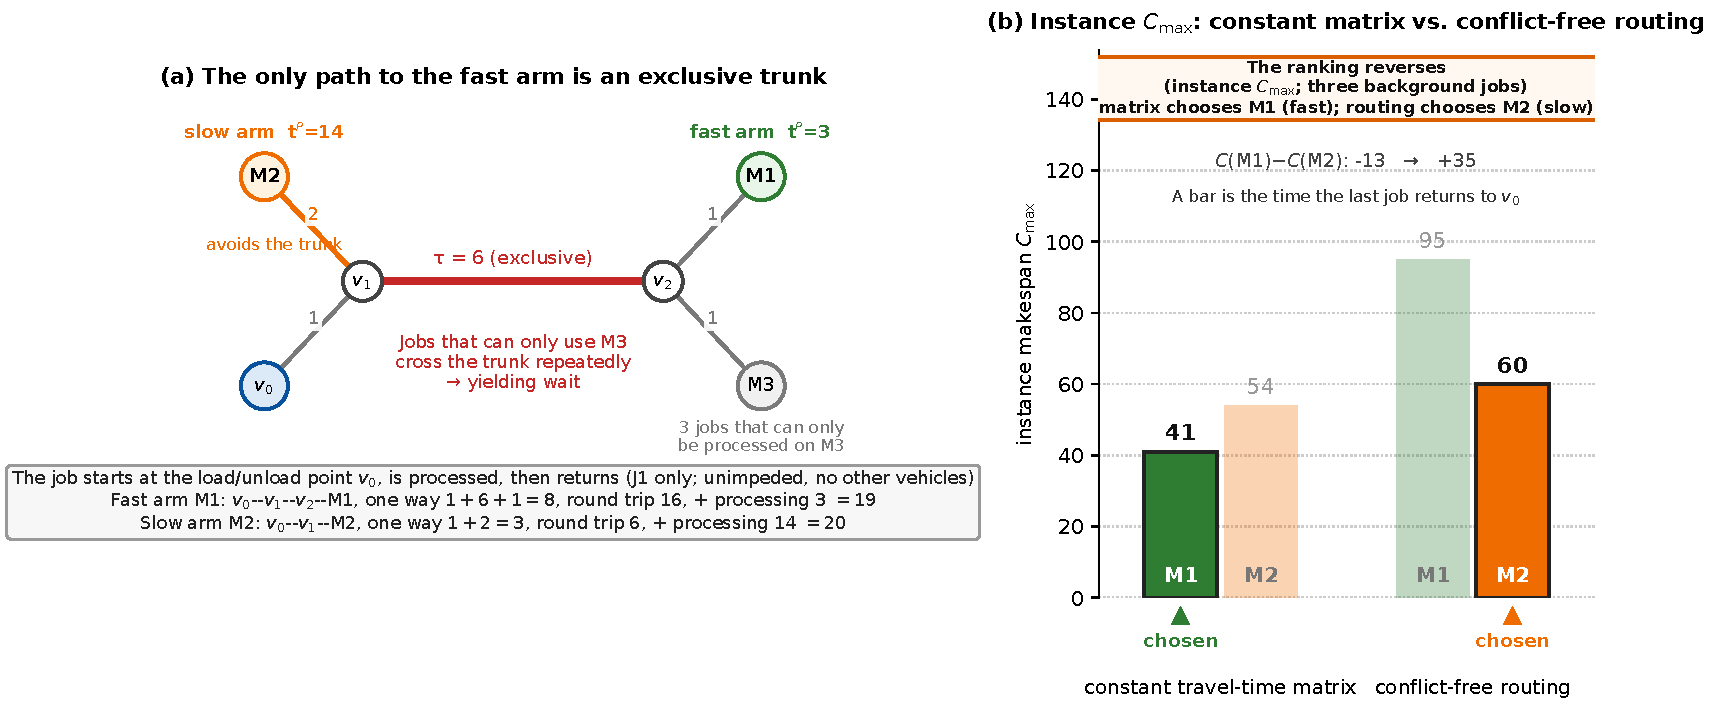
\includegraphics[width=\textwidth]{fig/fig_motivating.pdf}
\Description{Left: shop network with an exclusive trunk to the fast arm. Right: makespans of two assignments, 41 versus 54 under the constant matrix and 95 versus 60 under conflict-free routing.}
\caption{Motivating instance. (a)~Network: exclusive trunk ($\tau=6$) to the fast arm M1, short corridor to the slow arm M2, three M3-only jobs crossing the trunk. (b)~Instance makespan $C_{\max}$ of the two assignments of J1 under the constant matrix and under conflict-free routing. All times in dimensionless time units. Of $1200$ nearby parameter combinations, $205$ ($17\%$) show the reversal.}
\label{fig:motivating}
%% Generated by fig/fig_motivating.py from clbs/output/motivating.json (same decoder as the paper).
\end{figure}

Most existing work covers only part of this setting: scheduling with transportation uses a constant matrix, and conflict-free path planning takes task origins, destinations and release times as given.
\Citet{vanos2026exact} formalize the combined problem and solve small benchmark instances to proven optimality.
We focus on settings not previously taken as a dedicated object of study: transport longer than processing ($\bar{T}_t/\bar{T}_p\approx4.0$, against at most \PubTtTpHi{} on common public instances), corridors exclusive over their whole length, waiting only at berths, and congestion on a few shared corridors, with contention intensity as a controlled variable and sizes that exact decomposition has difficulty solving.
There, heuristics schedule first and resolve conflicts afterwards~\citep{sun2023integrated}, feed back realized durations once without reassignment~\citep{li2026framework}, or embed routing in decoding without measuring its benefit and cost~\citep{lyu2019approach}.
Under equal compute it is thus unmeasured how to trade off ``fast but congested'' against ``slow but clear'' arms, what counting yielding delay in the search gains, and at what contention this gain is worth its cost.

\subsection{Approach and contributions}

The upper level of our closed-loop bilevel framework decides machine assignment and operation sequencing; the lower level plans conflict-free paths by time-window reservation.
On the evaluation path, routing-in-the-loop evaluation ranks each candidate by its makespan after conflict-free routing, so yielding wait enters the search objective; such a decode costs over an order of magnitude more than one on unimpeded times, and neither \citet{li2026framework}, who list a fully iterative loop as future work, nor Lyu et al.\ report its cost or gain.
On the decision path, reservation-table-aware dispatching trial-queries both legs for each candidate vehicle on the current reservation table, without writing it, and selects the earliest feasible delivery instead of idle-first dispatching~\citep{lu2022agv}; admissible lower-bound pruning and winner-path reuse skip only trial queries that cannot affect the result.

A four-level baseline ladder forms a $2\times2$ design over whether the search counts conflict-induced delay and whether vehicles are chosen by unimpeded time or by trial query: B0 is the open-loop structure of constant-matrix methods and Li et al.\ on a real network, B0+ dispatches by the reservation table on a frozen schedule as in Sun et al., B1 closes the loop with rule-based dispatching, and B2 is our method.
All share the search, the router and the wall-clock budget, and are compared by realized makespan (Section~\ref{sec:protocol}).
With dispatching fixed, the closed loop reduces makespan by \GainLoopRule{} ($p\PLoopRule$) and remains significant on \CellsSigLoopAdj{} of the \NCases{} instances after Holm correction; within it, reservation-table-aware dispatching adds \GainProbeLoop{} ($p\PProbeLoop$) but is significant on no single instance; end to end, the reduction is \GainEndToEnd{} ($p\PEndToEnd$), slightly below the \GainIndepProduct{} predicted by independent composition (Section~\ref{sec:main}).
Our contributions are:

\begin{enumerate}[leftmargin=*]
\item \textbf{Controlled instances.} Instance families with controllable contention intensity let us examine how high contention must be before counting yielding wait in the schedule brings a gain (Section~\ref{sec:instances}).
\item \textbf{Routing-in-the-loop evaluation.} Its gain and cost over the open loop are measured at an equal wall-clock budget, and every chromosome decodes into a conflict-free, deadlock-free timetable without repair (Proposition~\ref{prop:decodable}).
\item \textbf{Low-overhead dispatching.} The speed-ups make each dispatching evaluation \SpeedupProbe{} times faster without changing the selected vehicle or the final timetable (Proposition~\ref{prop:speedup_equiv}), which makes a net gain possible at an equal budget.
\item \textbf{Decomposed evidence.} The closed loop is the larger effect and dispatching a much smaller one whose sign varies with the vehicle-to-arm ratio; the two do not amplify each other. An extra cost on occupied corridor--time slots (hereafter, surcharge) and yield-record-guided reassignment or staggering only add overhead; the failure of the surcharge suggests checking first whether the receiving level's objective already contains what an interface would pass.
\end{enumerate}

Sections~\ref{sec:Chapter_II}--\ref{sec:Chapter_V} cover related work, the problem (notation in Table~\ref{tab:notation}), the framework and the experiments; the final section concludes.


\section{Related work}
\label{sec:Chapter_II}

Related work comprises scheduling with transportation, conflict-free routing with exogenous tasks, and their integration; Table~\ref{tab:related} compares them with this paper.

\subsection{Scheduling with transport and conflict-free routing}

Flexible job shop scheduling with transportation (FJSP\_PT) brings material movement into the schedule (FJSP review~\citep{dauzereperes2024fjsp}; benchmarks~\citep{homayouni2021production}), and its dominant convention is a constant travel-time matrix, a fixed $t(a,b)$ regardless of corridor occupancy~\citep{xin2025review}.
Recent work keeps the matrix and improves solution methods: \citet{meng2025cp} close 29 open benchmark instances and improve 27 best-known solutions with constraint programming and a genetic algorithm; \citet{qin2026knowledge} use Q-learning and a local search guided by AGVs and the critical path; \citet{jafarian2026integrated} jointly optimize scheduling and internal logistics.
Vehicles thus never delay one another, and although critical-chain local search is mature~\citep{otala2021graph,tamssaouet2023neighborhood}, a critical path on the matrix leads back to an operation or a machine, not to a corridor; Xin et al.\ note that such assumptions ``even change [the problem's] nature'' and that $\bar{T}_t/\bar{T}_p$ is likely to affect algorithm performance.
% [ref_check: key=meng2025cp; claim="closes 29 open instances, improves 27 best-known solutions"; need=quote]

Optimal multi-agent path finding (MAPF) is NP-hard~\citep{gao2023mapf}, and \citet{kasaura2022sipp} extend Safe Interval Path Planning to continuous-time road networks.
For continuously arriving tasks, \citet{zhang2024guidance} optimize edge weights offline to steer agents away from bottlenecks, and \citet{kim2026congestion} propose congestion-aware dispatching rules for large AGV fleets; surveys~\citep{lu2022agv,fragapane2021planning} treat dispatching and path planning as separate layers.
Task release times and endpoints are inputs, so the router cannot revise the assignment, and congestion is measured indirectly (local density, offline edge weights), without identifying which transport caused yielding, when, and where.

\subsection{Integrated approaches and research gap}

\Citet{vanos2026exact} use logic-based Benders decomposition, whose integer-programming routing subproblem returns conflicts to a constraint-programming master as cuts; they solve most benchmarks to proven optimality and improve about half by at least 10\% over prior heuristics, but only at small scale, and list fuller use of ``which conflicts caused the infeasibility'' as future work.
\citet{sun2023integrated} fix the schedule by a hybrid genetic algorithm and then resolve conflicts by time-window Dijkstra, so congestion found later cannot change the schedule.
\citet{li2026framework} feed realized durations back once, shifting start times of the current solution without reassignment, with one eligible machine per operation.
\citet{lyu2019approach} route inside genetic-algorithm decoding, with vehicles encoded in the chromosome and conflicts resolved by local rules, but study fleet sizing on small instances, with neither an open-loop comparison nor a cost report.

The gap is thus not whether conflicts are handled but how routing results enter the schedule and what that is worth.
Beyond the reach of exact decomposition, and with corridors rather than nodes reserved, we route every candidate, dispatch by trial query, measure both contributions at an equal wall-clock budget, and vary contention intensity, since instances with the same $\bar{T}_t/\bar{T}_p$ may differ greatly in how much congestion reassignment can bypass.

\begin{table}[!htbp]
  \caption{Related work versus this paper. Het.: machine-dependent processing times on optional machines; Excl.: one vehicle per corridor at a time; transport times are unimpeded (ignoring other vehicles) or routed (with yielding wait); Gain/cost measured: closed-loop gain and cost measured against the open loop at equal compute.}
\label{tab:related}
%% Hand-maintained table: any row change must match Section 2.2.
\footnotesize
\renewcommand{\arraystretch}{1.05}
\begin{adjustbox}{max width=\linewidth}\begin{tabular}{@{}>{\raggedright\arraybackslash}p{2.3cm}>{\raggedright\arraybackslash}p{2.7cm}cc>{\raggedright\arraybackslash}p{2.6cm}c>{\raggedright\arraybackslash}p{2.6cm}@{}}
\toprule
Work class & Ref. & Het. & Excl. & Transport times used to evaluate schedules & \begin{tabular}[t]{@{}c@{}}Gain/cost\\measured\end{tabular} & Research focus \\
\midrule
FJSP\_PT metaheuristics & \citealp{meng2025cp,qin2026knowledge,jafarian2026integrated} & yes & no & unimpeded (matrix) & no & quality under a matrix \\
Lifelong MAPF & \citealp{gao2023mapf,zhang2024guidance} & --- & yes & none (tasks exogenous) & no & throughput \\
Congestion-aware dispatching & \citealp{kim2026congestion} & --- & no & none (tasks exogenous) & no & large-fleet congestion \\
Two-stage FJSP + routing & \citealp{sun2023integrated} & yes & yes & unimpeded; routed after freezing & no & schedule, then resolve \\
RL scheduling + PBS & \citealp{li2026framework} & no & yes & unimpeded; one correction & no & RL with multi-vehicle paths \\
GA + time-window routing & \citealp{lyu2019approach} & yes & yes & routed, every candidate & no & fleet size \\
Exact LBBD & \citealp{vanos2026exact} & yes & no & bound + conflict cuts & no & small-scale optimality \\
\textbf{This paper} & & yes & yes & routed, every candidate; trial-query dispatching & \begin{tabular}[t]{@{}c@{}}yes (equal\\wall clock)\end{tabular} & fast/slow-arm trade-off; closed-loop gain and cost \\
\bottomrule
\end{tabular}\end{adjustbox}
\end{table}
\section{Problem statement and model}
\label{sec:Chapter_III}
\subsection{Problem statement}

An instance consists of $n$ jobs, $N_M$ robotic arms, and $N_A$ vehicles (AGVs) on a shop-floor graph (Table~\ref{tab:notation}).
Job $j$ is a fixed chain of $n_j$ operations $O_{j1}\to\cdots\to O_{jn_j}$; operation $O_{ji}$ may be processed on any arm in its option set $\Omega_{ji}\subseteq M$, taking an arm-dependent time $t^P_{jim}$.
Arms occupy fixed nodes, and the fleet moves jobs between them.
Four decision groups are solved at once:
(i)~assign each operation to an arm in $\Omega_{ji}$;
(ii)~sequence the operations on each arm;
(iii)~assign the induced transport tasks to vehicles and sequence each vehicle's tasks;
(iv)~plan for every move a path that is conflict-free in time and space, waiting allowed.
The objective is to minimize the makespan $C_{\max}$.

\begin{table}[!htbp]
\caption{Notation.}
\label{tab:notation}
\footnotesize
\begin{adjustbox}{max width=\linewidth}\begin{tabular}{@{}ll@{}}
\toprule
Symbol & Meaning \\
\midrule
$J=\{1,\dots,n\}$, $O_{ji}$ & jobs; $i$-th operation of job $j$, $i\le n_j$ \\
$M=\{1,\dots,N_M\}$, $\Omega_{ji}\subseteq M$ & robotic arms; option set of $O_{ji}$ \\
$t^P_{jim}$ & processing time of $O_{ji}$ on arm $m\in\Omega_{ji}$ \\
$K=\{1,\dots,N_A\}$ & homogeneous unit-load vehicles \\
$G=(V,E)$, $\tau_e$ & shop-floor graph; traversal time of corridor $e$ \\
$v_0$, $\mathrm{loc}(m)$ & load/unload point; node of arm $m$ \\
$t^{*}(a,b)$ & shortest-path time $a\to b$ in $G$, ignoring contention \\
$\delta_{\mathrm{ret}}\in\{0,1\}$ & finished job returns to $v_0$ (baseline $1$) \\
$S_{ji}$, $C_{ji}$, $A_{ji}$, $C_{\max}$ & start, completion, material arrival; makespan \\
\bottomrule
\end{tabular}\end{adjustbox}
\end{table}

\subsection{Modelling assumptions}
\label{sec:assumptions}

\begin{enumerate}[label=\textbf{A\arabic*.},leftmargin=*,topsep=2pt,itemsep=1pt]
\item \textbf{Static instance and complete information.} All $n$ jobs are at $v_0$ at $t=0$; no release or due dates. Processing data, $G$, and vehicle states are known at planning time.

\item \textbf{Jobs.} Fixed precedence chain per job. Processing and transport are non-preemptive; jobs cannot be split; no exogenous precedence among jobs.

\item \textbf{Robotic arms: partial flexibility and heterogeneous times.} $O_{ji}$ may run on any $m\in\Omega_{ji}$ (most operations have $|\Omega_{ji}|\ge 2$; $\Omega_{ji}=M$ is a special case). Times $t^P_{jim}$ vary with the arm and need not be proportional across arms. An arm processes one operation at a time and does not fail; sequence-dependent setup is folded into $t^P_{jim}$.

\item \textbf{Buffers and loading.} Ample input/output buffers and storage at $v_0$, so no blocking. Loading and unloading are negligible and do not occupy the arm.

\item \textbf{Vehicles.} $N_A$ homogeneous unit-load vehicles at constant speed, empty or loaded; no acceleration or battery. All stand empty and available at $v_0$ at $t=0$. A task is a one-way move---$v_0$ to the first arm, between successive distinct arms, or, when $\delta_{\mathrm{ret}}=1$, last arm back to $v_0$; any vehicle may take any task, so a job's moves may be relayed across vehicles. After unloading, a vehicle is not forced back to $v_0$; it follows its own task chain, and routing may postpone its departure.

\item \textbf{Road network and conflict-freedom.} $G$ is strongly connected; each $\tau_e$ is a known constant. Corridors are \emph{exclusive}: both directions of $e$ share one reservation, so at most one vehicle occupies $e$ at a time (no head-on conflict, no overtaking). Occupancy is half-open, $[t,\,t+\tau_e)$, so a second vehicle may enter at $t+\tau_e$. Nodes have ample berths, separate from the traversal resource; waits occur at berths and are always permitted.

\item \textbf{Out of scope.} Machine and vehicle failures, finite buffers and blocking, battery charging, and dynamic job arrivals~\citep{gui2023dynamic,zhao2026deep} are left to future work (item~(5) of Section~\ref{sec:future_work}).
\end{enumerate}

A1, A2, A4, and A5 are standard in FJSP\_PT~\citep{xin2025review}; our problem is defined by A3 and A6, which make transport duration an output of routing rather than a constant matrix entry.
Deadlock-freedom is not assumed: Proposition~\ref{prop:decodable} uses A4 and A6 to prove that any assignment and sequence decodes into a conflict-free, deadlock-free timetable, so the search need not repair infeasible solutions.

\subsection{Decision variables and induced transport tasks}

Let $x_{jim}\in\{0,1\}$ indicate that $O_{ji}$ is assigned to arm $m$; write $\mathrm{m}(j,i)$ for the chosen arm and $d_{ji}=\mathrm{loc}(\mathrm{m}(j,i))$ for its node.
When $\delta_{\mathrm{ret}}=1$, a zero-duration dummy operation $O_{j,n_j+1}$ at $v_0$ represents the return, so return moves share the task notation and the makespan is always the completion of each job's last operation.
Unlike in vehicle routing, transport tasks are not an input but are \emph{induced} by the assignment:
\begin{equation}
\label{eq:tasks}
\mathcal{T}(x)=\Bigl\{\,(j,i)\ :\ d_{j,i-1}\neq d_{ji}\,\Bigr\},
\qquad d_{j0}\equiv v_0 ,
\end{equation}
where task $(j,i)$ moves job $j$ from $d_{j,i-1}$ to $d_{ji}$ and is ready at $r_{ji}=C_{j,i-1}$ ($C_{j0}=0$).
Decision~(i) thus fixes the number and endpoints of tasks: a job kept on one arm needs two moves, one that changes arm at every operation $n_j+1$.
Tasks are assigned to vehicles by $y_{tk}\in\{0,1\}$ with $\sum_{k\in K}y_{tk}=1$ for each $t\in\mathcal{T}(x)$, and each vehicle's tasks are sequenced.
A constant travel-time matrix model shares this dependence but treats move durations as constants; here the assignment also determines on which corridors the moves contend.

\subsection{Timing relations and feasibility}

With $p_{ji}=\sum_{m\in\Omega_{ji}}x_{jim}t^P_{jim}$, assignment, precedence, and unit arm capacity give
\begin{align}
\sum_{m\in\Omega_{ji}} x_{jim} &= 1, & \forall j,i,
\label{eq:assign}\\
C_{ji} &= S_{ji}+p_{ji}, & \forall j,i,
\label{eq:dur}\\
S_{ji} &\ \ge\ A_{ji}, & \forall j,i,
\label{eq:material}\\
S_{j'i'}\ \ge\ C_{ji}\ \ \vee\ \ S_{ji} &\ \ge\ C_{j'i'}
& \forall (j,i)\neq(j',i')\ \text{on the same arm},
\label{eq:disj}
\end{align}
where $A_{ji}$ is the time at which the job actually appears at $d_{ji}$: $A_{ji}=C_{j,i-1}$ if $(j,i)\notin\mathcal{T}(x)$; otherwise, with $a^{\mathrm{E}}_{ji}$ the time at which the carrying vehicle reaches the pickup node after its empty leg,
\begin{equation}
\label{eq:load}
\ell_{ji}=\max\bigl(a^{\mathrm{E}}_{ji},\ r_{ji}\bigr),
\quad
A_{ji}=\text{arrival time of the loaded leg departing at } \ell_{ji},
\end{equation}
so either may wait for the other.
Each leg, empty or loaded, is a walk $(e_1,\dots,e_q)$ in $G$ whose corridor entry times satisfy
\begin{equation}
\label{eq:walk}
\eta_1 \ \ge\ \sigma, \qquad
\eta_{l+1}\ \ge\ \eta_l+\tau_{e_l}, \quad l=1,\dots,q-1,
\end{equation}
where $\sigma$ is the earliest start of the leg; a strict inequality is a wait at a berth, and the leg ends at $\eta_q+\tau_{e_q}$.
Any two distinct occupancies of the same corridor $e$, regardless of direction and vehicle, satisfy
\begin{equation}
\label{eq:excl}
\bigl[\eta,\ \eta+\tau_e\bigr)\ \cap\
\bigl[\eta',\ \eta'+\tau_e\bigr)\ =\ \emptyset ,
\end{equation}
the only constraint that couples jobs through space rather than through a shared arm. The objective is
\begin{equation}
\label{eq:obj}
\min\ C_{\max},\qquad
C_{\max}=\max_{j\in J}\ C_{j,\,n_j+\delta_{\mathrm{ret}}} .
\end{equation}
In a semi-active schedule, Eqs.~\eqref{eq:material} and~\eqref{eq:disj} tighten to
\begin{equation}
\label{eq:bind}
S_{ji}=\max\bigl(A_{ji},\ F_{\mathrm{m}(j,i)}\bigr),
\end{equation}
where $F_m$ is the completion time of the operation immediately before $O_{ji}$ on arm $m$; Section~\ref{sec:Chapter_IV} uses this to attribute a postponed start to waiting for the workpiece or for the arm.

\subsection{Relation to FJSP\_PT}
\label{sec:fjsppt}

Without Eq.~\eqref{eq:excl}, every leg takes an unimpeded shortest path, durations collapse to the constant matrix $t^{*}(a,b)$ (later a lower bound and the open-loop arrival estimate), and the model becomes flexible job shop scheduling with transportation (FJSP\_PT); corridor exclusivity is the only difference.
\citet{vanos2026exact} reserve nodes, whereas we reserve edges in both directions; \citet{lyu2019approach} also reserve edges but allow one vehicle per node, whereas our nodes have ample berths (like the standby areas beside real workstations), so congestion occurs only on corridors.
Why the instances cannot be compared directly is limitation~(1) in Section~\ref{sec:limitations}.

\subsection{Computational complexity}

\begin{prop}
\label{prop:np_hard}
The problem defined by Eqs.~\eqref{eq:assign}--\eqref{eq:obj} is strongly NP-hard, and it remains so when every operation satisfies
$\Omega_{ji}=M$.
\end{prop}

\begin{proof}
Set $\tau_e=0$ for all $e$, give each arm a dedicated corridor from $v_0$, and let $N_A=n$: Eq.~\eqref{eq:excl} then holds trivially and $A_{ji}=C_{j,i-1}$, leaving Eqs.~\eqref{eq:assign}--\eqref{eq:disj}, the flexible job shop with unrelated machines~\citep{dauzereperes2024fjsp}.
Its special cases $|\Omega_{ji}|=1$ (classical job shop, three machines) and $\Omega_{ji}=M$, $n_j=1$ (unrelated parallel machines, machine count in the input) are strongly NP-hard, and each restriction is a polynomial reduction.
\end{proof}

Hardness thus holds even without contention; fixing decisions~(i)--(iii) still leaves conflict-free multi-agent routing~\citep{gao2023mapf}, so routing adds to the scheduling difficulty rather than replacing it.
Logic-based Benders decomposition solves most small benchmark instances of this setting to optimality~\citep{vanos2026exact}; we target larger sizes.

\subsection{Instance features}
\label{sec:features}

Size is fixed and only structure varies (size: limitation~(1), Section~\ref{sec:limitations}).
Four standard features are recorded: $\bar{T}_t/\bar{T}_p$, mean shortest-path travel between arm nodes over mean processing time, likely to affect performance~\citep{xin2025review}; heterogeneity $H$, the coefficient of variation of each operation's processing times over its optional arms, averaged (singletons count $0$), where larger $H$ leaves less room to reassign around congestion, so we do not expect the gain to rise with $H$ (Section~\ref{sec:whichcongestion}); flexibility $F=\operatorname{mean}_{ji}|\Omega_{ji}|/N_M$, the scope of reassignment; and $N_A/N_M$, small values favouring a transport bottleneck.
Two are specific to road networks: contention intensity, the share of travel time that is yielding wait on the initial random population, which orders the instances (Table~\ref{tab:instances}); and the funnel width $|\mathrm{cut}(v_0)|$, the size of a smallest corridor set separating $v_0$ from every arm, which bounds how many vehicles can leave $v_0$ at once (Family~A varies it; \texttt{funnel} halves the value of \texttt{high}).

The lower bound $\mathrm{LB}=\max(\mathrm{LB}_{\text{chain}},\mathrm{LB}_{\text{load}},\mathrm{LB}_{\text{cut}})$ combines a per-job chain bound (shortest inbound and return trips plus $\sum_i \min_m t^P_{jim}$), a load bound $\sum_{j,i}\min_m t^P_{jim}/N_M$, and a cut bound spreading the $X=2n$ crossings of $\mathrm{cut}(v_0)$ (when $\delta_{\mathrm{ret}}=1$) over its corridors:
\begin{equation}
\label{eq:lbcut}
C_{\max}\ \ge\ X\Bigl/\sum_{e\in \mathrm{cut}(v_0)}\tau_e^{-1}.
\end{equation}
$\mathrm{LB}_{\text{cut}}$ is largest on eight of our ten instances and $\mathrm{LB}_{\text{chain}}$ on the other two; the bound is loose (gap \LBGapLo{} to \LBGapHi{} to the best known solution) and serves only as a correctness check, since a solution below it signals an implementation error (Section~\ref{sec:protocol}); distance to the optimum is discussed in Section~\ref{sec:external} and limitation~(3), Section~\ref{sec:limitations}.

\section{Closed-loop bilevel framework}
\label{sec:Chapter_IV}
\subsection{Overview: routing-in-the-loop evaluation and the decision path}
\label{sec:overview}

The framework assigns the four decision groups to two levels (Figure~\ref{fig:framework}).
A memetic algorithm~\citep{zhang2024memetic} searches over assignment and sequencing; an event-driven decoder turns each candidate into transport tasks; and the lower level routes them conflict-free by time-window reservation, returning an executable timetable and its makespan.
Unlike two-stage or single-correction schemes, the framework differs in how routing enters the schedule: the content and direction of the feedback, and whether every candidate receives it.
On the \emph{evaluation path}, i.e.\ routing-in-the-loop evaluation, every candidate's fitness is its makespan after conflict-free routing, yielding wait included.
On the \emph{decision path}, reservation-table-aware dispatching picks each vehicle by a trial query on the reservation table rather than by unimpeded travel time.
Section~\ref{sec:Chapter_V} measures the two paths separately and reports control results for two further inter-layer interfaces (Section~\ref{sec:interface}): the surcharge on occupied corridor--time slots and the yield record.

%% 本图由 fig/fig_framework_CN.py 生成,是一张示意图,不含任何数据。
%% 注意不要复用 fig/fig_hdp_architecture*.pdf,那是上一篇论文的 HDP 框架。
\begin{figure}[!htbp]
\centering
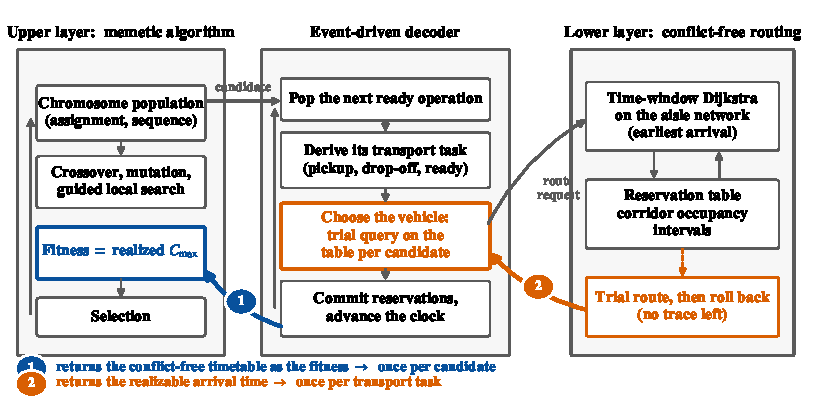
\includegraphics[width=\textwidth]{fig/fig_framework.pdf}
\caption{The closed-loop bilevel framework: memetic search (upper), event-driven decoder (middle), and time-window reservation routing (lower).
Path~1 (blue) returns the conflict-free timetable as fitness, once per candidate; path~2 (orange) runs a two-leg trial query before each vehicle choice, once per transport task, without writing the final timetable.
}
\Description{Schematic of the framework: an upper memetic search layer, an
event-driven decoder, and a lower reservation-based routing layer, with two
colour-coded feedback paths entering the upper layer at different places.}
\label{fig:framework}
\end{figure}

\subsection{Lower level: time-window reservation and conflict-free routing}
\label{sec:router}

The reservation table maps each corridor, the only contended resource (A6), to a time-ordered list of half-open occupancy intervals $[t,\,t+\tau_e)$ labelled by vehicle and task.
It supports four operations: earliest feasible entry no earlier than a given instant; write; revoke a task; and checkpoint and rollback around a trial query.
Nodes take zero time and waits occur at berths, so nodes are not reserved, and both the conflict-free path planner (hereafter, the router) and an independent checker inspect only corridor occupancy.

The router is a time-window Dijkstra search (Algorithm~\ref{alg:route}) whose label $(u,t)$, with cost $t$, means standing at the berth of $u$ at time $t$.
For each corridor leaving $u$ the table returns the earliest feasible entry $t'\ge t$, so the berth wait $t'-t$ of Eq.~\eqref{eq:walk} is produced by the search itself.
Written paths are not revoked within a decode, so vehicles are planned in task-generation order and a later-planned vehicle yields to an earlier one.

\begin{lem}[One earliest-arrival label per node suffices]
\label{lem:label}
Keeping only the earliest-arrival label at each node is sufficient to obtain a path that reaches the destination earliest under the current reservation table.
\end{lem}

\begin{proof}
Ample berths occupy no corridor (A6), so a vehicle at $u$ since $t$ can wait until any $s>t$ and take every continuation open to one arriving at $s$; an earlier label is never worse.
With $R.\textsc{EarliestEntry}(e,t,\tau_e)$ the earliest conflict-free entry into $e$ no earlier than $t$, later queries see no more free slots, so the exit time $t\mapsto R.\textsc{EarliestEntry}(e,t,\tau_e)+\tau_e$ is non-decreasing; labels leave the queue in increasing time, so the first extraction of the destination is the earliest arrival.
\end{proof}

Ordinary Dijkstra therefore suffices, without the per-interval labelling of Safe Interval Path Planning (SIPP)~\citep{kasaura2022sipp}; a second criterion such as a surcharge would require a multi-label search (Section~\ref{sec:interface}).

\begin{algorithm}[!htbp]
  \caption{\textsc{Route}: conflict-free planning of a single leg}
  \label{alg:route}
  \footnotesize
  \begin{algorithmic}[1]
  \Require $s$, $g$, departure $t_0$, table $R$, flag \textit{commit}
  \State push $(s,t_0)$ onto a queue keyed by (time, node id)
  \While{the queue is nonempty}
    \State pop the least label $(u,t)$
    \If{$u=g$} \State backtrack occupancies; write them if \textit{commit}; \Return $t$ \EndIf
    \ForAll{corridors $e=(u,v)$}
      \State $t_{\text{in}} \gets R.\textsc{EarliestEntry}(e,t,\tau_e)$; update $(v,\,t_{\text{in}}+\tau_e)$ if strictly earlier
    \EndFor
  \EndWhile
  \State \Return failure \Comment{unreachable; see text}
  \end{algorithmic}
\end{algorithm}

A path always exists because reservations are finite and $G$ is strongly connected: at worst the vehicle waits until every occupancy has ended, then takes an unimpeded shortest path.
With $W$ the mean number of intervals per corridor, a call costs $O\bigl(|E|\,(W^{2}+\log|V|)\bigr)$ ($O(W)$ candidate entries per corridor, each tested in $O(W)$); a logarithmic earliest-entry query would give $O\bigl(|E|(\log W+\log|V|)\bigr)$, but we use the linear scan.
On an empty table the search yields $t^{*}$, used for open-loop estimates, the reassignment proximity term, the two-stage baseline, and the pruning bound (Section~\ref{sec:speedup}).

\subsection{Upper level: encoding and event-driven decoding}
\label{sec:upper}

An individual has two segments: a machine-assignment vector whose $k$-th entry is the arm chosen from $\Omega_{ji}$ for the $k$-th of the $N$ operations, and an operation sequence in which job $j$ appears $n_j$ times (plus once for its dummy when $\delta_{\mathrm{ret}}=1$), its $x$-th appearance standing for $O_{jx}$; operations sharing an arm are ordered by the sequence.
Vehicles are chosen at decode time (Section~\ref{sec:dispatch}), since a third segment would enlarge the search space and lose guaranteed decodability.

The decoder (Algorithm~\ref{alg:decode}) implements the evaluation path.
Sweeping the sequence, it generates a task of Eq.~\eqref{eq:tasks} whenever an operation's arm differs from the job's location, chooses a vehicle, and plans the empty and loaded legs against the live table, joined by Eq.~\eqref{eq:load}.
The operation starts by Eq.~\eqref{eq:bind}, and the recorded \texttt{bind} field (waiting for the workpiece or for the arm) is authoritative for later tracing of postponed starts.

\begin{algorithm}[!htbp]
\caption{\textsc{Decode}: fitness from a complete conflict-free simulation}
\label{alg:decode}
\footnotesize
\begin{algorithmic}[1]
\Require assignment $x$, operation sequence
\State $F_m,\mathrm{ready}_j,\mathrm{avail}_k\gets 0$; $\mathrm{pos}_j,\mathrm{loc}_k\gets v_0$; clear $R$
\ForAll{$O_{ji}$ in sequence order (dummies included)}
  \State $d\gets \mathrm{loc}(m)$ for the arm $m$ of $O_{ji}$ under $x$
  \If{$\mathrm{pos}_j=d$} \State $A_{ji}\gets \mathrm{ready}_j$
  \Else
     \State choose vehicle $k$ (Section~\ref{sec:dispatch}); $a^{\mathrm{E}}\gets\textsc{Route}(\mathrm{loc}_k,\mathrm{pos}_j,\mathrm{avail}_k,R,\text{true})$
     \State $A_{ji}\gets\textsc{Route}(\mathrm{pos}_j,d,\max(a^{\mathrm{E}},\mathrm{ready}_j),R,\text{true})$; $\mathrm{loc}_k,\mathrm{avail}_k\gets d,A_{ji}$
     \State accumulate yielding time by corridor
  \EndIf
  \State $\texttt{bind}\gets\texttt{machine}$ if $F_m>A_{ji}$, else $\texttt{arrive}$
  \State $S_{ji}\gets\max(A_{ji},F_m)$; $C_{ji}\gets S_{ji}+p_{ji}$; $F_m,\mathrm{ready}_j\gets C_{ji}$; $\mathrm{pos}_j\gets d$
\EndFor
\State \Return $\max_{j,i} C_{ji}$, timetable, yield statistics
\end{algorithmic}
\end{algorithm}

Decoding is deterministic: reservations are written in task-generation order, the routing queue breaks ties by node id and updates a label only on a strictly earlier arrival, and dispatching scans vehicles by increasing id and keeps the first strictly better one.
A chromosome thus maps to a unique timetable, on which the seed-paired, equal-budget comparisons of Section~\ref{sec:Chapter_V} depend.

\begin{prop}[Every chromosome is decodable]
  \label{prop:decodable}
  For any machine assignment and any operation sequence, Algorithm~\ref{alg:decode} terminates and returns a conflict-free, deadlock-free timetable of finite makespan. The search therefore need not invoke a repair operator.
\end{prop}

\begin{proof}
The sequence is a topological order of each job's chain, so $\mathrm{ready}_j$ is known when read, and ample buffers (A4) let Eq.~\eqref{eq:bind} give a finite start once the job has arrived.
Each \textsc{Route} call terminates by the existence argument after Algorithm~\ref{alg:route} and occupies only free slots, so Eq.~\eqref{eq:excl} holds by construction.
Deadlock cannot occur: the corridor is the only contended resource (A6), waits occupy only ample berths, and every written occupancy ends at a finite time, so no circular wait arises.
The sweep runs $N+n\delta_{\mathrm{ret}}$ times, each scheduling finitely many events at finite times.
\end{proof}

\subsection{Reservation-table-aware dispatching}
\label{sec:dispatch}

The open-loop rule scores each vehicle by its unimpeded-shortest-path delivery estimate,
\begin{equation}
\label{eq:rule}
\mathrm{score}(k)=\max\bigl(\mathrm{avail}_k+t^{*}(\mathrm{loc}_k,\text{pickup}),\,
\mathrm{ready}_j\bigr)+t^{*}(\text{pickup},\text{destination}),
\end{equation}
the idle-first dispatching of \citet{li2026framework} and a typical single-attribute rule in multi-AGV dispatching~\citep{lu2022agv}; ignoring the reservation table, it may pick a nearby vehicle whose corridors are already occupied.
The closed-loop default, reservation-table-aware dispatching, runs a trial query per candidate vehicle: the empty leg is planned and temporarily written (otherwise both legs could share a corridor--time slot and the result would be too early), the loaded leg is planned against that state, the earliest feasible delivery is recorded, and the table is rolled back.
The vehicle with the earliest feasible delivery is selected; since vehicles are identical (A5) and differ only in location and corridor occupancy, contention on the table can directly determine the choice.
The cost is up to $2N_A$ instead of $2$ routing calls per task, about \CostMultBefore{} times the evaluation cost of rule-based dispatching; unless reduced (Section~\ref{sec:speedup}), this overhead offsets the makespan gain under an equal wall-clock budget, so Section~\ref{sec:Chapter_V} compares the two rules only under the same wall-clock limit.

\subsection{Low overhead: admissible lower-bound pruning and winner-path reuse}
\label{sec:speedup}

At equal generations reservation-table-aware dispatching beats rule-based dispatching by \GainProbeSameGen{}, but at equal wall-clock time its \CostMultBefore{}-fold evaluation cost leaves a net effect close to zero; the two speed-ups below reduce this multiple without changing any selection.

\paragraph{Admissible lower-bound pruning.}
Yielding can only delay routing, never beat the shortest path that ignores contention, so the open-loop estimate of Eq.~\eqref{eq:rule} is an admissible lower bound on the realized delivery time:
\begin{equation}
\label{eq:lb_dispatch}
\begin{split}
\mathrm{lb}(k)={}&\max\bigl(\mathrm{avail}_k+t^{*}(\mathrm{loc}_k,\text{pickup}),\,\mathrm{ready}_j\bigr)\\
&+t^{*}(\text{pickup},\text{destination})\ \le\ \mathrm{est}(k),
\end{split}
\end{equation}
where $\mathrm{est}(k)$ is the earliest feasible delivery from a complete two-leg trial query for vehicle $k$.
A vehicle whose bound is no earlier than the best trial-query delivery so far needs no routing call.

\paragraph{Winner-path reuse.}
Rollback discards the winner's two legs, which the decoder would replan on the same restored table; as routing is deterministic, the cached trial-query paths are written directly, saving two calls.

\begin{prop}[The two speed-ups do not change the selected vehicle or the timetable]
  \label{prop:speedup_equiv}
  In the implementation, vehicles are queried in increasing id order, and the selected vehicle is replaced only when some vehicle's feasible delivery is strictly earlier than the current best.
  Under this rule, after the pruning of Eq.~\eqref{eq:lb_dispatch} and winner-path reuse are added, the selected vehicle, the occupancies written to the reservation table, and the final timetable are the same as when a complete two-leg trial query is run for every vehicle.
\end{prop}

\begin{proof}
If $\mathrm{lb}(k)\ge\mathrm{est}^{\ast}$, the current best, then $\mathrm{est}(k)\ge\mathrm{lb}(k)\ge\mathrm{est}^{\ast}$ by Eq.~\eqref{eq:lb_dispatch}, so $k$ is not strictly earlier and would not be selected anyway; pruned vehicles write nothing to the table, which is restored after each trial query, so later queries are unaffected.
The winner's legs were computed against the very table state the decoder writes into after restoration, and routing is deterministic, so cached and replanned paths give identical occupancies.
\end{proof}

Jointly, measured as one on/off switch (Table~\ref{tab:prune}) and not attributed to pruning or reuse separately, the speed-ups give a \SpeedupProbe{}-fold speed-up, cut routing calls by \RouteCallCut{}, and reduce the cost multiple from \CostMultBefore{} to \CostMultAfter{}.
Trial-query cost grows roughly linearly with $N_A$, and pruning weakens as the fleet grows yet still cuts \RouteCallCutLo{} of the calls on the largest fleet tested; the gain may thus vanish beyond some fleet size, which the present number of seeds is not sufficient to determine (Section~\ref{sec:whichcongestion}).

\subsection{Two further inter-layer interfaces: surcharges and yield records}
\label{sec:interface}\label{sec:ls}

Both paths read realized durations, i.e.\ traversal times after conflict-free routing, for every candidate, whereas schedule-then-route methods obtain them once, after the assignment is fixed.
Realized durations do not reveal which decision caused a wait, so we implement two richer interfaces and compare them under an equal wall-clock budget (Section~\ref{sec:pricing}).

A \emph{surcharge} $\pi(e,b)$, by analogy with shadow prices in Lagrangian relaxation and column generation, is added to arrival time by a vehicle occupying corridor $e$ in slot $b$: routing minimizes arrival time $+\,\theta\cdot$ the surcharges traversed (the surcharge coefficient $\theta\ge0$ is the only tunable parameter), and reassignment likewise pays for its traversals.
$\pi$ is estimated by perturbing one slot's capacity and re-solving, or by a low-cost approximation refreshed each generation.
While fitness comes from a complete conflict-free decode, such a cost adds no information: contention wait already enters arrival time, makespan (Eq.~\eqref{eq:bind}) and fitness, so the surcharge counts it twice, and blocking of later tasks already shows in the decoded makespan; we verify this inference on this one interface only.
By Lemma~\ref{lem:label}, the second criterion also forces a multi-label Pareto search, raising evaluation cost whether or not the surcharge is non-zero.

A \emph{yield record} instead returns structure: the triple (corridor, time slot, preceding occupying transport) that routing knows at each yield.
It enters no objective, so no delay is double-counted; it only shapes the neighbourhood of yield-record-guided local search, applied with the same setting to the top-ranked individuals of each generation in all four main-batch configurations.
The search backtracks from the makespan-determining event along a critical chain that includes transport legs, since a wait for the workpiece may stem from an upstream operation, a missing vehicle, or contention; links are labelled as in Table~\ref{tab:attrib}, a yield on a loaded leg counting as \texttt{corridor} and an empty leg classified by whether yielding exceeds half its duration.
For each of at most $L=5$ real operations on the chain, reassignment yields one neighbour by moving it from arm $m$ to the arm $m'\in\Omega_{ji}\setminus\{m\}$ minimizing
\begin{equation}
\label{eq:reassign}
\mathrm{score}(m')=t^{*}\bigl(d_{j,i-1},\mathrm{loc}(m')\bigr)+t^{P}_{jim'},
\end{equation}
trading a longer processing time for a shorter path with better traffic (cumulative yield, a fleet- and horizon-wide total, is not commensurable and is omitted).
Staggering advances the blocked operation or postpones the preceding occupier on the longest \texttt{corridor} link by swapping adjacent appearances of different jobs, preserving decodability (Proposition~\ref{prop:decodable}).
The first improvement among these at most $L+2=7$ neighbours is accepted, for at most three rounds with the chain recomputed each round; the same tracing reads the case study (Section~\ref{sec:casestudy}).

\begin{table}[!htbp]
\caption{Critical-chain link labels and remedies. Only \texttt{corridor} names a corridor, time slot, and preceding transport.}
\label{tab:attrib}
\footnotesize
\begin{adjustbox}{max width=\linewidth}\begin{tabular}{@{}llp{2.3cm}@{}}
\toprule
Label & Criterion & Remedy \\
\midrule
\texttt{operation} & a real operation occupies its arm & --- \\
\texttt{machine} & waiting for the arm & resequence \\
\texttt{upstream} & vehicle first, material not ready & recurse to $O_{j,i-1}$ \\
\texttt{vehicle} & material ready, vehicle late, little yielding & change vehicle \\
\texttt{corridor} & yield on a given corridor and slot & reassignment or staggering \\
\bottomrule
\end{tabular}\end{adjustbox}
\end{table}

\subsection{Outer genetic algorithm, complexity and cost}

The outer layer is a conventional genetic algorithm: a random initial population plus a fastest-arm and a greedy load-balancing individual; tournament selection with a small elite; precedence-preserving order crossover on the sequence, uniform crossover on the assignment; and swap or reassignment mutation (hyperparameters in Section~\ref{sec:impl}).

One evaluation processes $N+n\delta_{\mathrm{ret}}$ events with at most $2N_A$ routing calls per transport under closed-loop dispatching, so an individual costs $O\bigl((N+n)\,N_A\,|E|\,(W^{2}+\log|V|)\bigr)$; open-loop selection drops the factor $N_A$.
The speed-ups leave this bound and every selection unchanged (Proposition~\ref{prop:speedup_equiv}) but cut routing calls by \RouteCallCut{} (\RouteCallCutLo{} to \RouteCallCutHi{} across instances), in effect shrinking $N_A$; local search adds at most $3(L+2)=21$ decodes per selected individual.
On the ladder batch one evaluation takes \MsOpen{}\,ms open-loop, \MsLoopRule{}\,ms with rule-based dispatching, and \MsLoopProbe{}\,ms full closed-loop (about $37$ times open-loop); in an earlier scan the surcharge raised it from \MsPricedRef{}\,ms to \MsPriced{}\,ms (about $4.8$ times), so costs span about two orders of magnitude, although the two batches' timings are not directly comparable.
A costlier evaluation buys fewer evaluations, so whether an interface pays off must be measured, and Section~\ref{sec:Chapter_V} aligns wall-clock time rather than generations.

These results guarantee correctness, not solution quality: Proposition~\ref{prop:decodable}, Lemma~\ref{lem:label}, and Proposition~\ref{prop:speedup_equiv} ensure that every candidate is feasible, that its evaluation matches the conflict model of Section~\ref{sec:Chapter_III}, and that the speed-ups change no selection, and deterministic decoding makes the procedure reproducible.
As with most metaheuristics, solution quality has no theoretical bound and is evaluated experimentally in the next section.
\section{Experiments}
\label{sec:Chapter_V}

This section measures the gains of the closed loop and of reservation-table-aware dispatching and whether they amplify each other, asks on which instances they hold and whether the present seeds can resolve this, and explains why the other interfaces yield no net gain.

\subsection{Experimental setup}
\label{sec:instances}

\subsubsection{Controlled instance families}
FJSP\_PT benchmarks write travel times as a matrix and supply no corridor network.
Of the \PubNLayout{} layouts of \citet{homayouni2021production}, \PubNLayoutAsym{} matrices are entirely asymmetric, ruling out undirected corridors, and \PubNLayoutBad{} also violate the triangle inequality, which no graph's shortest paths do; a network reverse-engineered from them would be a different instance.
We therefore generate controlled instances on an explicit road network, so that each feature of Section~\ref{sec:features} can be varied on its own; public instances, with contention removed, calibrate only the upper-level search (Section~\ref{sec:external}).

All instances share the core of Table~\ref{tab:instances}, with $\bar{T}_t/\bar{T}_p$ scaled so that vehicle contention is the main constraint and $H$ standardized per operation so that $F$ does not change it.

\emph{Family A: layout.}
In a spine layout a main corridor (the spine) runs through the arm area and each arm hangs off it on its own branch corridor, as in high-volume plants where congestion on the central corridor is a known problem~\citep{suh2022spine}.
Placing $v_0$ at one end of the spine, rather than where trips are balanced as real shops do, sends every transport through the same exit and corridor stretch: a deliberately high-contention construction, and exactly the case the closed loop targets.
Parallel lanes of equal duration change capacity, not distance; a tandem single-vehicle loop~\citep{rahimikelarijani2020tandem} has almost no contention.
\texttt{funnel}, \texttt{high}, and \texttt{mid} differ only in their lanes; \texttt{funnel} and \texttt{high} differ by one exit at $v_0$, halving the minimum cut, a single-factor contrast.
The grids \texttt{low} and \texttt{scatter} (arms at the farthest points) cover the low-contention range, but their farthest unimpeded trip is \LegGrid{} against \LegDumbbell{}, so only differences among the spine instances are attributable to capacity.
Contention intensity (\ContentionAHi{} to \ContentionLo{}) broadly decreases in this order but not strictly, as the grid \texttt{low} (\ContentionALow{}) is slightly above the spine \texttt{mid} (\ContentionAMid{}); the paper-wide maximum \ContentionHi{} is the $F=1.0$ instance of Family~C.

\emph{Family B} varies the vehicle-to-arm ratio on \texttt{funnel} to test whether dispatching has an upper limit in fleet size; \emph{Family C} varies flexibility, the fraction of arms each operation may use.
Their shared base point \texttt{A funnel} is run once, so $5+3+2=\NCases$, and must be counted when reading Families~B and~C.
Contention intensity is measured on the initial random population because optimized solutions route around congestion and erase the differences among instances.
Relative to the \PubNInst{} public instances compiled by \citet{homayouni2021production}, our base $F$ is about one and a half times the median \PubFMed{}, $H$ exceeds the maximum \PubHMax{} (median \PubHMed{}), and $\bar{T}_t/\bar{T}_p$ deliberately exceeds the maximum \PubTtTpHi{}; whether the high $H$ inflates the closed-loop gain is tested in Section~\ref{sec:whichcongestion}.

\begin{table}[!htbp]
\caption{Controlled instances. Shared core: $12$ jobs, $36$ real operations, $8$ arms, $H=0.3$, $\bar{T}_t/\bar{T}_p\approx4.0$.
Contention intensity: share of yielding wait in travel time on the initial random population.}
\label{tab:instances}
\small
%% 由 tab/gen_tables_ladder.py 生成:结构列直接由 tools/abc_matrix.py 的 build() 构造出
%% 算例后读出,下界调 algorithm/instance.py 的 simple_lower_bound,争用强度取自
%% baseline_ladder.csv 的 contention 列。任何一列都不是手打的。
%% 由 tab/gen_tables_ladder.py 生成,请勿手工编辑
%% 数据源:clbs/output/baseline_ladder.csv 等,见脚本首部
\begin{adjustbox}{max width=\linewidth}\begin{tabular}{@{}llrrrrrr@{}}
\toprule
Instance & Varied factor & Nodes & Corridors & $N_A$ & $F$ & Contention & Composite LB (time units) \\
\midrule
A funnel & layout & 13 & 12 & 12 & 0.61 & 31.9\% & 24.0 \\
A high & layout & 14 & 14 & 12 & 0.61 & 30.9\% & 17.0 \\
A low & layout & 16 & 24 & 12 & 0.61 & 11.8\% & 36.0 \\
A mid & layout & 15 & 16 & 12 & 0.61 & 10.8\% & 17.0 \\
A scatter & layout & 16 & 24 & 12 & 0.61 & 6.6\% & 36.0 \\
\midrule
B NA/NM 0.5 & $N_A/N_M$ & 13 & 12 & 4 & 0.61 & 15.8\% & 24.0 \\
B NA/NM 1.0 & $N_A/N_M$ & 13 & 12 & 8 & 0.61 & 30.2\% & 24.0 \\
B NA/NM 2.0 & $N_A/N_M$ & 13 & 12 & 16 & 0.61 & 32.4\% & 24.0 \\
\midrule
C F=0.3 & flexibility & 13 & 12 & 12 & 0.30 & 27.7\% & 24.0 \\
C F=1.0 & flexibility & 13 & 12 & 12 & 1.00 & 33.5\% & 24.0 \\
\bottomrule
\end{tabular}\end{adjustbox}

\end{table}

\subsubsection{Comparison protocol}
\label{sec:protocol}

Every schedule is executed by the same conflict-free router and checked against the composite lower bound by a validator independent of the decoder; failing runs are reported separately.
We compare realized makespans, because the open loop's self-reported makespan is often infeasible; the gap (hereafter, the optimism margin) is especially large on the funnel layout.
One evaluation costs up to about two orders of magnitude more in some configurations than in others, so configurations share an equal wall-clock budget (Table~\ref{tab:batches}) rather than a generation count, with early stopping after $400$ generations without improvement.
Every open-loop run stops early, using about one fifth of the budget, while both closed-loop configurations use all of it; this favours the baseline, which completes as many evaluations as closed-loop rule-based dispatching, or more (Section~\ref{sec:costlaw}).

\begin{table}[!htbp]
\caption{Experiment batches; only the main batch supports Tables~\ref{tab:main} and~\ref{tab:bytag}. Speed-ups: pruning and winner-path reuse (Section~\ref{sec:speedup}).}
\label{tab:batches}
\footnotesize
\begin{adjustbox}{max width=\linewidth}\begin{tabular}{@{}>{\raggedright\arraybackslash}p{2.3cm}>{\raggedright\arraybackslash}p{3.2cm}>{\raggedright\arraybackslash}p{2.1cm}c>{\raggedright\arraybackslash}p{2.4cm}c@{}}
\toprule
Batch & Purpose & Instances & Seeds & Wall-clock budget & Speed-ups \\
\midrule
Main & Ladder (Tables~\ref{tab:main}, \ref{tab:bytag}) & Ten controlled & $\NSeeds$ & $90$\,s & yes \\
Cost diagnosis & Figure~\ref{fig:protocol} & Three controlled & $3$ & $90$\,s & yes \\
Convergence diagnosis & Optimism margin (Section~\ref{sec:main}) & \texttt{funnel} & $3$ & $46.3$\,s & yes \\
Speed-up switch & Table~\ref{tab:prune} & Six controlled & $10$ & $90$\,s & off/on \\
Budget convention & Section~\ref{sec:costlaw} & Four & $10$ & Equal wall-clock; equal generations & no \\
Surcharge scan & Section~\ref{sec:pricing} & Two $8\times4\times4$ & $10$/$5$ & $48.9$/$60.7$\,s & no \\
Independent instances & Cross-check, $H$, ablations (Sections~\ref{sec:whichcongestion}, \ref{sec:pricing}) & $\MatrixCells$ & $10$ & $30.2$--$72.9$\,s & no \\
Public benchmarks & Table~\ref{tab:external} & $\PubNInst$ public & $\NSeeds$ & Early stopping & --- \\
\bottomrule
\end{tabular}\end{adjustbox}
\end{table}

Three seeds on one instance spanned $11$ makespan units, more than any mechanism effect, so each instance runs $\NSeeds$ seeds ($\NPairs$ pairs), compared by a two-sided Wilcoxon signed-rank test paired by seed; this resolves a few-percentage-point effect when pooled, not within one instance.
Since ten uncorrected tests give at least one false positive with probability about $40\%$, each family is Holm-corrected: the five pooled contrasts of Table~\ref{tab:main}, and the $\NCases$ instances of each effect in Table~\ref{tab:bytag} (Benjamini--Hochberg disagreements are marked).
Two marked exceptions stay uncorrected: the vehicle-to-arm-ratio $p$-values, which are already non-significant before correction and can only grow under it, and the significant-instance counts of the independent \MatrixCells{}-instance batch, whose instances and baselines differ from the main batch and which corroborate direction and magnitude only, supporting no conclusion.
Pooled contrasts also give a Hodges--Lehmann pseudomedian with a $95\%$ distribution-free interval from the test's null distribution, whereas the tabulated mean pairwise relative gain carries no precision; for dispatching in the closed loop the mean is \GainProbeLoop{} and the pseudomedian \HLProbeLoop{}, because pairs on two vehicle-to-arm-ratio instances worsen.
Figure error bars are standard errors of the mean.

\subsubsection{Implementation and environment}
\label{sec:impl}
Experiments run single-threaded on an Intel Xeon W-1270 @ $3.40$\,GHz in pure Python ($\ge 3.9.6$) without a solver, with untuned default hyperparameters shared by all configurations: population $60$, crossover $0.8$, mutation $0.2$, elite $5$, binary tournament; local search on the top $10\%$, at most $L=5$ critical operations per round, three rounds.
Compiled code would raise every configuration's evaluation count, not the cost ratios between them.

\subsection{Four-level baseline ladder}
\label{sec:arms}

Ablations alone cannot be mapped onto the pipeline structures of the literature, while a literature comparison alone would credit the gain of conflict-free routing itself to our mechanisms; the ladder serves both purposes as a $2\times2$ design (Table~\ref{tab:arms}).
\textbf{B0} searches on unimpeded shortest-path times and executes the plan with the same router and idle-first dispatching (Eq.~\eqref{eq:rule}); constant-matrix FJSP\_PT methods~\citep{meng2025cp,qin2026knowledge,jafarian2026integrated} executed on a real road network, and the framework of \citet{li2026framework}, fall into this class.
\textbf{B0+} keeps that schedule and changes only vehicle selection to a trial query on the reservation table, a greedy approximation of the second stage of two-stage structures such as \citet{sun2023integrated}.
\textbf{B1} takes fitness from conflict-free routing but dispatches by Eq.~\eqref{eq:rule}; \textbf{B2}, our method, differs from B1 only in vehicle selection.
$\text{B0+}\to\text{B1}$ changes both factors and cannot measure the closed loop.

\begin{table}[!htbp]
\caption{The $2\times2$ structure of the four-level ladder. Row or column contrasts change one factor; diagonal contrasts cannot be decomposed.}
\label{tab:arms}
\footnotesize
\begin{adjustbox}{max width=\linewidth}\begin{tabular}{@{}>{\raggedright\arraybackslash}p{6.4cm}>{\centering\arraybackslash}p{2.6cm}>{\centering\arraybackslash}p{3.2cm}@{}}
\toprule
 & Rule-based dispatching & Reservation-table-aware dispatching \\
\midrule
Open loop (schedule first, then route; search ignores conflicts) & B0 & B0+ \\
Closed-loop planning (fitness from conflict-free routing) & B1 & \textbf{B2} (ours) \\
\bottomrule
\end{tabular}\end{adjustbox}
\end{table}

B0 either \emph{replays the plan} with its specified vehicles or reassigns them on site. Replay is stronger ($63.00$ versus $78.00$ on the funnel instance) and matches \citet{li2026framework}, whose execution only shifts the Gantt chart in time; it is the main report, with on-site reassignment listed alongside.

\subsection{Aggregate comparison on the ladder}
\label{sec:main}

Table~\ref{tab:main} reports the ladder on $\NPairs$ pairs ($\NCases$ instances $\times$ $\NSeeds$ seeds); every run passed the independent check, and Holm correction over the five contrasts changes no decision.
The text states Hodges--Lehmann intervals as reductions; the table shows them as negative values.

\begin{table}[!htbp]
\caption{Four-level ladder under an equal wall-clock budget, and the four one-factor contrasts. Negative is better.
$n=\NPairs$ pairs on $(\text{instance},\text{seed})$; two-sided Wilcoxon signed-rank, Holm-corrected over the five contrasts
($^{*}p<0.05$, $^{**}p<0.01$, $^{***}p<0.001$). HL: Hodges--Lehmann pseudomedian with $95\%$ interval.
Bold marks our configuration, not a per-instance winner.}
\label{tab:main}
\small
%% 由 tab/gen_tables_ladder.py 从 clbs/output/baseline_ladder.csv 生成。该脚本同时打印
%% 导言区的整块宏定义,故表与正文的数字必然同源:重跑实验后只需重跑脚本、贴一次宏。
%% 已核实脚本独立复现出导言区当前的全部数值(增益、p 值、胜负计数、争用区间)。
%% 2026-08-20:p 列改为 Holm 校正后的值,并加印 HL 伪中位数与 95% CI。校正对这五个对比是
%% 惰性的:最大的一个 p 恰为最大者、乘数为 1,其余小到乘 5 仍远低于阈值,故数字不变而口径变严。
%% 由 tab/gen_tables_ladder.py 生成,请勿手工编辑
%% 数据源:clbs/output/baseline_ladder.csv 等,见脚本首部
\begin{adjustbox}{max width=\linewidth}\begin{tabular}{@{}lrrrrr@{}}
\toprule
& & \multicolumn{4}{c}{$C_{\max}$ (time units)} \\
\cmidrule(lr){3-6}
Instance & Contention & B0 & B0$^{+}$ & B1 & \textbf{B2} \\
\midrule
A funnel & 31.9\% & 58.10 & 53.50 & 44.70 & 42.40 \\
A high & 30.9\% & 56.00 & 51.40 & 39.90 & 37.70 \\
A low & 11.8\% & 64.50 & 64.60 & 57.80 & 57.10 \\
A mid & 10.8\% & 46.40 & 42.70 & 39.40 & 37.40 \\
A scatter & 6.6\% & 62.30 & 62.30 & 57.20 & 57.10 \\
\midrule
B NA/NM 0.5 & 15.8\% & 71.00 & 70.50 & 69.00 & 65.10 \\
B NA/NM 1.0 & 30.2\% & 56.70 & 56.50 & 47.50 & 49.80 \\
B NA/NM 2.0 & 32.4\% & 70.60 & 64.20 & 42.20 & 44.20 \\
\midrule
C F=0.3 & 27.7\% & 74.30 & 69.50 & 51.60 & 47.30 \\
C F=1.0 & 33.5\% & 52.10 & 47.50 & 39.30 & 36.30 \\
\midrule
\emph{Pooled mean} & --- & 61.20 & 58.27 & 48.86 & 47.44 \\
\bottomrule
\end{tabular}\end{adjustbox}

\vspace{0.6em}

\begin{adjustbox}{max width=\linewidth}\begin{tabular}{@{}lrlrr@{}}
\toprule
Single-factor paired contrast & $\Delta C_{\max}$ & HL pseudomedian and $95\%$ CI (\%) & W/L/T & $p_{\mathrm{Holm}}$ \\
\midrule
Closed-loop value (rule-based) & $-18.86\%^{***}$ & $-18.28$ $[-21.95,-14.68]$ & 96/2/2 & $<10^{-4}$ \\
Closed-loop value (reservation-table-aware) & $-17.75\%^{***}$ & $-18.00$ $[-20.55,-15.22]$ & 93/5/2 & $<10^{-4}$ \\
Dispatching value (open-loop) & $-4.59\%^{***}$ & $-4.45$ $[-6.13,-2.88]$ & 68/19/13 & $<10^{-4}$ \\
Dispatching value (closed-loop) & $-2.45\%^{**}$ & $-3.03$ $[-5.19,-0.94]$ & 60/34/6 & $0.0054$ \\
\midrule
\textbf{End-to-end: literature $\rightarrow$ this paper} & $-21.35\%^{***}$ & $-21.20$ $[-24.46,-17.99]$ & 94/5/1 & $<10^{-4}$ \\
\bottomrule
\end{tabular}\end{adjustbox}

\end{table}

With the vehicle-selection rule fixed, the closed loop is significantly better under both rules: $\text{B0}\to\text{B1}$ is $-\GainLoopRule$ ($p\PLoopRule$) and $\text{B0+}\to\text{B2}$ is $-\GainLoopProbe$ ($p\PLoopProbe$), so the conclusion does not depend on our dispatching rule.
For the former the pseudomedian is \HLLoopRule{} with interval \CILoopRule{}; even its lower end is a two-digit reduction.
The number of evaluations runs the other way: looking up a constant matrix, the open loop completes several times as many evaluations within the same budget (Figure~\ref{fig:protocol}) and is still worse, because it optimizes a surrogate that excludes yielding.
On a \texttt{funnel} diagnostic run (Table~\ref{tab:batches}) it converges, but to a surrogate value its plan cannot realize after execution: the optimism margin.

With the loop fixed, reservation-table-aware dispatching inside the closed loop gives $\text{B1}\to\text{B2}$ of $-\GainProbeLoop$ ($p\PProbeLoop$; pseudomedian \HLProbeLoop{}, interval \CIProbeLoop{}), with search and budget shared.
This is a pooled result: the interval excludes zero by less than one percentage point, no instance is significant after correction (\CellsSigProbe{} before), and at vehicle-to-arm ratios $1.0$ and $2.0$ B2 is slower than B1 (Table~\ref{tab:bytag}).
$-\GainProbeLoop$ is therefore an average over this instance family, not an instance-level estimate.
Under the open loop the same rule gives $-\GainProbeOpen$ ($p\PProbeOpen$), likewise significant; it measures the step from the open-loop to the two-stage structure and is far smaller than the closed loop's \GainLoopRule{}.
Dispatching is thus significant under both loops but much smaller, and cannot by itself explain the end-to-end reduction.

\paragraph{End to end, and how the two effects combine.}
\label{sec:complement}
Pooled, $\text{B0}\to\text{B2}$ is $-\GainEndToEnd$ ($p\PEndToEnd$; $\WinEndToEnd$ wins, $\LoseEndToEnd$ losses, and $1$ tie among $\NPairs$ pairs), about one fifth of the makespan.
The effects have different reference points and cannot be added directly: were the mechanisms independent, the compound of \GainLoopRule{} (closed loop, rule-based dispatching) and \GainProbeOpen{} (dispatching, open loop) would be \GainIndepProduct{}, and the measured \GainEndToEnd{} is slightly below it.
Each mechanism contributes on its own and \emph{the two do not amplify each other}; B2 is best end to end because the gains add up.
This also locates the shortfall of ``schedule first, then resolve conflicts'': second-stage dispatching gains only \GainProbeOpen{}, far less than \GainLoopRule{}, so the shortfall lies in the first stage ignoring yielding, and the closed-loop reduction requires yielding wait in the fitness during the search. These gaps were measured on our instance families.

\subsection{Three-factor scans and per-instance resolution}
\label{sec:whichcongestion}

The three families test whether the gains grow with contention intensity, whether trial-query overhead, growing with the fleet while the pruning of Section~\ref{sec:speedup} weakens, caps the dispatching gain, and whether the gains need room for reassignment.
With Holm correction over the $\NCases$ instances of one effect (all marks in Table~\ref{tab:bytag} and Figure~\ref{fig:prediction3}), the closed loop remains significant on \CellsSigLoopAdj{} instances (\CellsSigLoop{} uncorrected; largest corrected value $p\PLoopCellMax$), all but the instance with the fewest vehicles (\GainLoopStarve{}, not significant), so it can be read by family.
Dispatching is significant on \CellsSigProbe{} instances before correction, the two ends of the flexibility family ($p\PProbeFlexLoRaw$, $p\PProbeFlexHiRaw$), and on \CellsSigProbeAdj{} after it (Holm $p\PProbeFlexLoHolm$, $p\PProbeFlexHiHolm$; Benjamini--Hochberg $p\PProbeFlexLoBH$, $p\PProbeFlexHiBH$): its few-percentage-point effect is near the smallest that $\NSeeds$ seeds resolve on one instance, and only the $\NPairs$ pooled pairs reach significance, and only narrowly.
Its per-instance results are therefore directions only.

\begin{table}[!htbp]
\caption{Per-instance ladder results and the two effects, by family ($n=\NSeeds$ seed pairs per instance). Marks: Holm-corrected two-sided Wilcoxon over the $\NCases$ instances of one effect, $^{*}p<0.05$, $^{**}p<0.01$; $^{\dagger}$ significant only before correction. Negative is better; gains are means of pairwise relative gains, as in Table~\ref{tab:main}.
\texttt{A funnel} also serves as $N_A/N_M=1.5$ and $F=0.6$.}
\label{tab:bytag}
\small
%% 由 tab/gen_tables_ladder.py 生成,按 A/B/C 三族分块。
%% 逐格增益列已于 2026-08-16 从"两档均值之比"改为"逐对相对增益的均值",与 tab_main 及
%% 导言区宏同源;同时加印显著性标记,因为下文按格读符号。
%% 标记已于 2026-08-20 改按 Holm 校正后的 p 值,并为"校正前显著、校正后不显著"的格加印
%% 剑号。改动只影响标记,不影响任何增益数字;受影响的格是柔性族两格(试探列)。
%% 由 tab/gen_tables_ladder.py 生成,请勿手工编辑
%% 数据源:clbs/output/baseline_ladder.csv 等,见脚本首部
\begin{adjustbox}{max width=\linewidth}\begin{tabular}{@{}lrrrrrrr@{}}
\toprule
& & \multicolumn{4}{c}{$C_{\max}$ (time units)} & \multicolumn{2}{c}{Pairwise relative gain} \\
\cmidrule(lr){3-6}\cmidrule(lr){7-8}
Instance & Contention & B0 & B0$^{+}$ & B1 & \textbf{B2} & B0$\rightarrow$B1 & B1$\rightarrow$B2 \\
\midrule
A funnel & 31.9\% & 58.10 & 53.50 & 44.70 & 42.40 & $-21.3\%^{*}$ & $-4.6\%$ \\
A high & 30.9\% & 56.00 & 51.40 & 39.90 & 37.70 & $-26.6\%^{*}$ & $-4.8\%$ \\
A low & 11.8\% & 64.50 & 64.60 & 57.80 & 57.10 & $-10.3\%^{*}$ & $-1.1\%$ \\
A mid & 10.8\% & 46.40 & 42.70 & 39.40 & 37.40 & $-14.4\%^{*}$ & $-4.8\%$ \\
A scatter & 6.6\% & 62.30 & 62.30 & 57.20 & 57.10 & $-8.1\%^{*}$ & $+0.1\%$ \\
\midrule
B NA/NM 0.5 & 15.8\% & 71.00 & 70.50 & 69.00 & 65.10 & $-2.0\%$ & $-4.7\%$ \\
B NA/NM 1.0 & 30.2\% & 56.70 & 56.50 & 47.50 & 49.80 & $-15.6\%^{*}$ & $+5.0\%$ \\
B NA/NM 2.0 & 32.4\% & 70.60 & 64.20 & 42.20 & 44.20 & $-37.7\%^{*}$ & $+5.7\%$ \\
\midrule
C F=0.3 & 27.7\% & 74.30 & 69.50 & 51.60 & 47.30 & $-29.7\%^{*}$ & $-8.2\%^{\dagger}$ \\
C F=1.0 & 33.5\% & 52.10 & 47.50 & 39.30 & 36.30 & $-22.9\%^{*}$ & $-7.2\%^{\dagger}$ \\
\bottomrule
\end{tabular}\end{adjustbox}

\end{table}

\begin{figure}[!htbp]
\centering
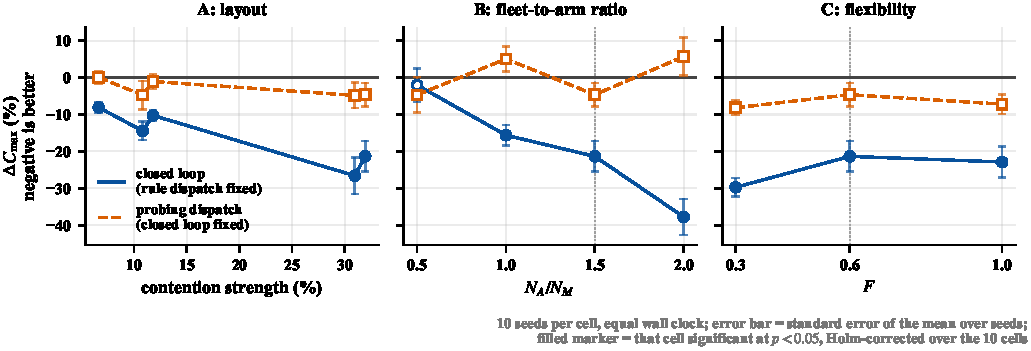
\includegraphics[width=\textwidth]{fig/fig_prediction3.pdf}
\Description{Three panels of line plots: closed-loop gain and reservation-aware
dispatch gain across layout (vs contention), fleet-to-arm ratio, and flexibility. After
Holm correction over the ten cells the closed-loop curve is filled, hence
significant, at nine of ten cells, while the dispatch curve is hollow at every
cell, and its sign alternates across the four fleet-ratio levels. Error bars
give the standard error of the mean over the ten seeds of each cell; the
dispatch bars cross zero at every cell and the closed-loop bars do not.}
\caption{Closed-loop and dispatching gains by family: layout against contention intensity (left), $N_A/N_M$ (middle), flexibility (right); vertical lines mark the base point \texttt{A funnel}.
Filled markers: significant after Holm correction over the $\NCases$ instances of one effect. Error bars: standard error over $\NSeeds$ seeds.}
\label{fig:prediction3}
%% 由 fig/fig_prediction3_CN.py 从 clbs/output/baseline_ladder.csv 生成。横轴:A 族取争用强度
%% (布局族没有自然的数值水平,而布局操纵改变的正是争用),B/C 族取算例名末尾的因子水平——
%% 那个数字由 tools/abc_matrix.py 生成算例时写入,故按构造即为水平本身;基点 A funnel 的
%% 名字里没有水平,其 (1.5, 0.6) 由脚本按 abc_matrix.BASE 显式补入,见脚本内注释。
%% 标记的实心/空心由逐格 Wilcoxon 的 p 值决定。上一版按增益是否为正标注 "harmful",
%% 那等于把不显著的符号当成结论,现已改为按显著性区分标记。
%% 2026-08-20:填充判据改为 Holm 校正后的 p 值,族取该效应的全部十格(而不是当前面板的
%% 三到五格,否则共用基点会因所在面板不同而得到两种填充)。改动后试探那条曲线全为空心。
\end{figure}

In the layout family the closed loop is significant on all five instances and rises roughly with contention, from \GainLoopScatter{} on \texttt{scatter} (\ContentionLo{}) through \GainLoopMid{}/\GainLoopLow{} on \texttt{mid}/\texttt{low} to \GainLoopFunnel{}/\GainLoopHigh{} on \texttt{funnel}/\texttt{high}.
Two inversions qualify this: \texttt{low} versus \texttt{mid} straddles the topological boundary, but \texttt{funnel} versus \texttt{high} is the planned single-factor contrast, so \emph{this inversion is a counter-example}.
What is established is the magnitude, about two and a half times larger on the most congested instance than on the least, not a monotone relation between contention and gain; contention intensity does not separate the congestion that reassignment can bypass (Limitation~(1), Section~\ref{sec:limitations}).
Dispatching is significant on no instance here; four of five signs match the closed loop.

The vehicle-to-arm-ratio family does not establish an upper bound for dispatching: from $N_A/N_M=0.5$ to $2.0$ it is $-\GainProbeStarve$, \GainProbeFleetOne{}, \GainProbeFleetBase{}, and \GainProbeFleetTwo{}, alternating in sign and non-significant even before correction ($p\PProbeFleetHalfRaw$, $p\PProbeFleetOneRaw$, $p\PProbeFleetBaseRaw$, $p\PProbeFleetTwoRaw$).
Without the base point the curve would show the rise predicted by the cost law, so the upper bound of Section~\ref{sec:costlaw} remains untested; testing it needs more seeds than our budget allows.
The closed loop stays significant at $1.0$ and $2.0$ (\GainLoopFleetOne{}, \GainLoopFleetTwo{}): fleet size mainly affects the closed-loop gain.

In the flexibility family dispatching is \GainProbeFlexLo{}, \GainProbeFleetBase{}, and \GainProbeFlexHi{}, all with the pooled sign; the two ends are the largest magnitudes but lose significance after correction.
Since $F=0.3$, with the least room for reassignment, has the largest magnitude, dispatching appears to act through vehicle selection and timing rather than reassignment.
The closed loop is \GainLoopFlexLo{} and \GainLoopFlexHi{}, significant after correction.

\paragraph{Independent batch and heterogeneity.}
A separate batch of contended self-generated instances ($\MatrixRuns$ runs; Table~\ref{tab:batches}) crosses four contention levels with four $H$ levels against a two-stage surrogate-transport baseline.
Its \emph{integration gain} (two-stage $\to$ closed loop), \GainIntegMatrix{}, significant on \SigIntegMatrix{} instances (uncorrected), matches the closed loop here in direction and magnitude.
By $H$ level it is \GainIntegHZero{} at $H=0$, \GainIntegHLow{} at $0.15$ (measured \MatrixHMeasLow{}, near the public median \PubHMed{}), \GainIntegHMid{} at $0.3$, and \GainIntegHHigh{} at $0.5$, with a weakly negative rank correlation \RhoIntegH{}.
Setting $H$ above the literature range thus did not raise the gain; with four instances per level and a within-level spread (\GainIntegMatrixLo{} to \GainIntegMatrixHi{}) far exceeding the gaps between levels, the data support only that the gain does not rise with $H$, not that $H=0.5$ is lower.
As Section~\ref{sec:features} predicts, a larger $H$ lets processing speed rather than traffic decide assignment, while $H=0$ makes reassignment a pure congestion decision and has the highest gain; $H$ creates the trade-off behind the reversal of Section~\ref{sec:Chapter_I} but does not amplify the closed-loop gain.
For dispatching this batch gives \GainProbePre{} ($0$ instances significant), opposite to the main batch; it ran before the two speed-ups (Section~\ref{sec:costlaw}).
\subsection{Ablations and controlled negative controls}
\label{sec:pricing}

The surcharge is off by default ($\theta=0$), and yield-record-guided local search runs with the same setting in all four configurations, so neither affects the comparisons between them.

On the $\MatrixCells$-instance batch of Section~\ref{sec:whichcongestion}, valid here because the cost of these operators, unlike that of dispatching, does not depend on pruning, turning off yield-record feedback gives a relative gain of \GainCertMatrix{} (significant on $1$ instance) and turning off staggering gives \GainStaggerMatrix{} (significant on $2$). Neither is positive: under an equal wall-clock budget, these decodes are better spent on population evolution. The local search consumes a large share of all decodes, yet fewer than one in fifty of its neighbours improve makespan although the neighbourhood is small and well targeted (Section~\ref{sec:ls}), and three refinements of its operators were each not significant under an equal number of evaluations, so the signal itself fails.

The surcharge counts again a delay that fitness already includes (Section~\ref{sec:interface}), so it adds no information, but its cost must be measured. On two instances outside Families A/B/C (Table~\ref{tab:batches}), with the path-planning search width fixed, every surcharge coefficient $\theta$ tried worsens makespan significantly at equal wall-clock time, flat over a ten-fold range, whereas at an equal number of evaluations the difference is not significant. Routing with a surcharge completes only about one fifth as many evaluations, because a second criterion removes total-order dominance (Lemma~\ref{lem:label}) and requires a multi-label search whose overhead is the same at every $\theta$. Nor is $\theta$ a useful tuning parameter: the cumulative surcharge is too small to reorder arrivals, so makespan is unchanged over two orders of magnitude until the surcharge outweighs the arrival time and the double counting worsens it sharply. An interface that passes a quantity already contained in the objective of the receiving layer is therefore harmful under our protocol.

\paragraph{Dilution and overhead.}
\label{sec:whycost}
A yield record names what is needed to remove one corridor delay, but makespan is set by a chain: once that delay is removed, another constraint usually becomes tight, so makespan improves by far less than the yielding time removed. The same dilution leaves reservation-table-aware dispatching only a few percentage points, not significant at a cost multiple of \CostMultBefore{} and significant in the pooled data once Section~\ref{sec:speedup} lowered it to \CostMultAfter{}. Local search thus fails because too little reduction survives dilution, whereas dispatching initially failed because each evaluation cost too much; dispatching is therefore a mechanism contribution, and yield-record-guided local search only a controlled negative control.


\subsection{The cost law and the effect of the two speed-ups}
\label{sec:costlaw}

Under a fixed wall-clock budget, the cost per evaluation and the number of evaluations trade off against each other (Figure~\ref{fig:protocol}): the cost spans about two orders of magnitude, and the open loop completes the most evaluations in about one fifth of the wall-clock time. An equal number of generations lets a costlier configuration use more compute and asks whether extra routing improves the ranking within a generation; equal wall-clock time asks whether makespan falls within the same time. The two conventions disagree: before the speed-ups, reservation-table-aware dispatching is \GainProbeSameGen{} ($p\PProbeSameGen$) at equal generations but only \GainProbeSameClock{} ($p\PProbeSameClock$) at equal wall-clock time, so we report both.

\begin{figure}[!htbp]
\centering
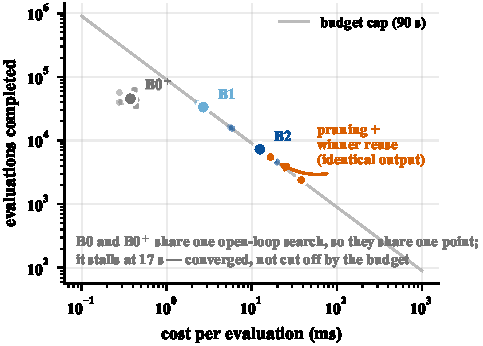
\includegraphics[width=0.7\columnwidth]{fig/fig_protocol.pdf}
\Description{A log-log scatter of cost per evaluation against evaluations
completed, with a grey hyperbola for the 90-second budget cap and orange
markers for the pruning ablation.}
\caption{Cost per evaluation against evaluations completed under the shared $90$-second cap (grey hyperbola).
The closed-loop configurations use the full budget; the open loop (B0 and B0$^+$ share one point) is ended by early stopping after about $17$\,s.
Pale points: three instances; filled points: their geometric mean. Orange: pruning and winner-path reuse off and on.}
\label{fig:protocol}
%% From fig/fig_protocol.py; ladder_cost.csv and prune_ablation.csv.
%% fig:protocols (two-convention comparison) dropped; the pair
%% \GainProbeSameGen / \GainProbeSameClock is reported in the text.
\end{figure}

The cost law follows from the trial query: it raises the routing calls per transport task from $2$ to at most $2N_A$, so cost grows linearly with fleet size, while pruning cuts fewer calls as fleet and contention grow (\RouteCallCutHi{} on the least congested self-check instance, \RouteCallCutLo{} on the largest fleet). The law predicts a fleet size beyond which the trial-query cost offsets the gain; across the four vehicle-to-arm levels of Section~\ref{sec:whichcongestion} the sign alternates and no instance is significant, so the law is measured but this bound is not confirmed.

Because the dispatching rule and the speed-ups were introduced one after the other, a separate control changes only pruning and winner-path reuse, with the same instances, seeds and budget. They change neither the selected vehicle nor the timetable (Proposition~\ref{prop:speedup_equiv}): for six random chromosomes on each of six instances, makespans and dispatch sequences are identical bit for bit in all $36$ cases while routing calls fall by \RouteCallCut{}, so any difference comes only from the compute saved. Switching them on lowers makespan by a further \GainPrune{} ($p\PPrune$; Table~\ref{tab:prune}). The same rule thus moves from \GainProbePre{} before the speed-ups ($0$ of the $\MatrixCells$ instances significant) to significantly positive after them, without any change of selection.

\begin{table}[!htbp]
\caption{Pruning and winner-path reuse off versus on (bold: adopted setting). Same instances, seeds and wall-clock time; $n=60$ pairs, two-sided Wilcoxon signed-rank test ($^{***}p<0.001$). Ratios take the off value as denominator.}
\label{tab:prune}
\small
%% Regenerated from prune_ablation.csv by gen_tables_ladder.py.
%% 由 tab/gen_tables_ladder.py 生成,请勿手工编辑
%% 数据源:clbs/output/baseline_ladder.csv 等,见脚本首部
\begin{adjustbox}{max width=\linewidth}\begin{tabular}{@{}lrrrrrr@{}}
\toprule
& & \multicolumn{2}{c}{$C_{\max}$ (time units)} & & Eval.\ count ratio & Speedup per eval. \\
\cmidrule(lr){3-4}
Instance & Contention & Off & \textbf{On} & $\Delta C_{\max}$ & (on/off) & (off/on) \\
\midrule
A funnel & 31.9\% & 44.80 & 42.10 & $-6.03\%$ & 2.21$\times$ & 2.23$\times$ \\
A high & 30.9\% & 41.60 & 37.70 & $-9.37\%$ & 2.40$\times$ & 2.41$\times$ \\
A low & 11.8\% & 60.50 & 57.00 & $-5.79\%$ & 2.79$\times$ & 2.81$\times$ \\
B NA/NM 0.5 & 15.8\% & 66.70 & 65.10 & $-2.40\%$ & 2.11$\times$ & 2.11$\times$ \\
B NA/NM 1.0 & 30.2\% & 51.90 & 48.90 & $-5.78\%$ & 2.31$\times$ & 2.31$\times$ \\
B NA/NM 2.0 & 32.4\% & 44.50 & 42.20 & $-5.17\%$ & 1.98$\times$ & 2.01$\times$ \\
\midrule
\emph{Pooled} (60 pairs) & --- & --- & --- & $-5.60\%^{***}$ & \multicolumn{2}{r}{50/0/10,\ $<10^{-4}$} \\
\midrule
\multicolumn{7}{@{}l@{}}{\footnotesize HL pseudomedian and $95\%$ CI:$-4.72$ $[-6.34,-3.55]$\,\%} \\
\bottomrule
\end{tabular}\end{adjustbox}

\end{table}

\subsection{Case study: Gantt chart and critical chain on the funnel instance}
\label{sec:casestudy}

Aggregate numbers do not show what happens inside one solve, so Figure~\ref{fig:case} places B0 and B2 side by side on one funnel instance.
In the open-loop solution, yielding waits cluster on the corridors near the load/unload point $v_0$ and on a few vehicles. The closed-loop solution greatly reduces them and assigns several operations to an arm that is not the fastest (Eq.~\eqref{eq:reassign}), trading a longer processing time for a less congested path; its more even vehicle load follows from these two effects rather than from a separate mechanism.
Labelled as in Table~\ref{tab:attrib}, the B0 critical chain contains a substantial share of \texttt{corridor} links; on B2 they largely give way to \texttt{machine} and \texttt{upstream} links, the dilution of Section~\ref{sec:whycost}.

\begin{figure}[!htbp]
\centering
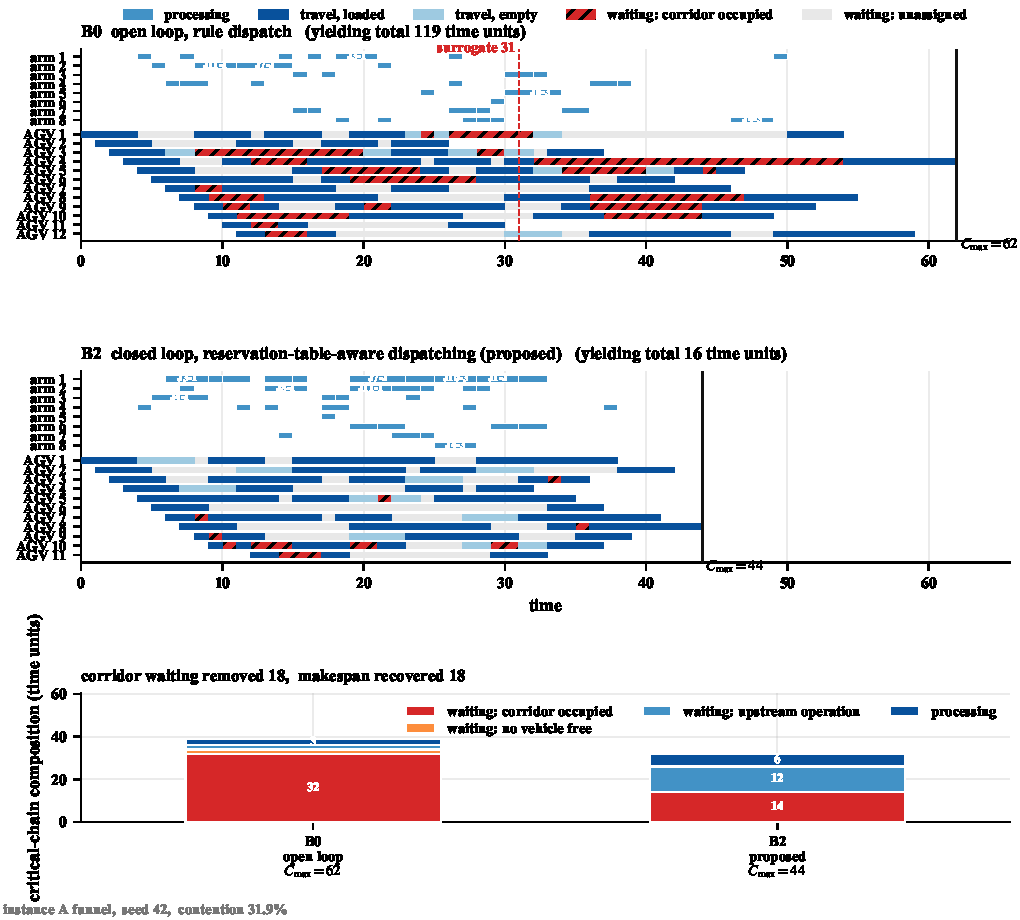
\includegraphics[width=\textwidth]{fig/fig_case.pdf}
\Description{Gantt charts of the open-loop and closed-loop solutions on one
funnel instance, followed by stacked bars decomposing each critical chain by
attribution label.}
\caption{B0 and B2 on one funnel instance.
Top: arms and vehicles on a shared time axis, with empty and loaded legs; a gap between the two legs of one transport is a yielding wait at a berth, a gap between tasks is idle time.
Bottom: critical-chain composition by the labels of Table~\ref{tab:attrib}, with corridor wait removed and makespan reduced.}
\label{fig:case}
%% From fig/fig_case.py and case_study/*.json (ladder_diag.py --case-study).
%% Merges the former fig_case_gantt / fig_case_chain pair.
\end{figure}

\subsection{Degenerate comparison on public benchmarks}
\label{sec:external}

Comparisons between configurations of one implementation cannot calibrate its absolute level. Without the exclusivity constraint, Eq.~\eqref{eq:excl}, and with $\delta_{\mathrm{ret}}=0$ (Table~\ref{tab:notation}), our model is exactly FJSP\_PT (Section~\ref{sec:Chapter_III}), the \emph{same mathematical problem} as the public benchmarks; neither mechanism is then active, so this anchors the upper-level search, not the framework. We use the \PubNInst{} instances of \citet{homayouni2021production} (from \citet{fattahi2007mathematical}) with two vehicles as in \citet{lim2023twophase}, and their published travel matrices as $t^{*}$, since \PubNLayoutBad{} are not a shortest-path closure (Section~\ref{sec:instances}); lacking a road network, they admit only this degenerate setting. References are MILP optima for \PubNOpt{} instances~\citep{homayouni2021production} and best published values for $4$~\citep{lim2023twophase}.

All $200$ runs pass validation and never fall below the composite lower bound or a proven optimum. On $\PubNMatch{}/\PubNInst{}$ instances, including all $10$ small ones, the best solution equals the reference digit for digit (Table~\ref{tab:external}); the mean gap is \PubGapMean{}, rising to \PubGapBig{} on the four largest. This reflects search capability, not budget: \PubBudgetRatio{} times the wall-clock time lowers the mean gap of the $10$ \textsc{mfjst} instances only from \PubGapLoBudget{} to \PubGapHiBudget{}, and all runs end by early stopping. On the proven-optimum instances the bound lies a median \PubLBSlack{} below the optimum while the search is at most $\PubLBResidMax$ percentage points above it, so without contention the bound gap is almost entirely bound slack. Since contention can only raise the optimum, the median bound gap of \LBGapMed{} on the self-generated instances \emph{cannot} be read as a search gap.

\begin{table}[!htbp]
\caption{Degenerate comparison on public benchmarks (exclusivity removed). \textsc{opt}: MILP-proven optimum; \textsc{bk}: best published value; gap from the best of \NSeeds{} seeds; asterisk: identical to the reference.}
\label{tab:external}
\centering
\small
%% 由 tab/gen_tables_ladder.py 生成,请勿手工编辑
%% 数据源:clbs/experiments_database/gap_ideal.csv;工序数取自 clbs/database/json/hf/*.json
\begin{adjustbox}{max width=\linewidth}\begin{tabular}{lrrrrrr}
\toprule
& & & \multicolumn{3}{c}{$C_{\max}$ (time units)} & \\
\cmidrule(lr){4-6}
Instance & Ops & Ref. & \multicolumn{1}{c}{Value} & Best & Mean & Gap \\
\midrule
SFJST01 & 4 & \textsc{opt} & 70 & 70\rlap{$^*$} & 70.0 & 0.00\% \\
SFJST02 & 4 & \textsc{opt} & 111 & 111\rlap{$^*$} & 111.0 & 0.00\% \\
SFJST03 & 6 & \textsc{opt} & 223 & 223\rlap{$^*$} & 223.0 & 0.00\% \\
SFJST04 & 6 & \textsc{opt} & 359 & 359\rlap{$^*$} & 359.0 & 0.00\% \\
SFJST05 & 6 & \textsc{opt} & 123 & 123\rlap{$^*$} & 123.0 & 0.00\% \\
SFJST06 & 9 & \textsc{opt} & 324 & 324\rlap{$^*$} & 324.0 & 0.00\% \\
SFJST07 & 9 & \textsc{opt} & 409 & 409\rlap{$^*$} & 409.0 & 0.00\% \\
SFJST08 & 9 & \textsc{opt} & 269 & 269\rlap{$^*$} & 269.5 & 0.00\% \\
SFJST09 & 9 & \textsc{opt} & 220 & 220\rlap{$^*$} & 222.0 & 0.00\% \\
SFJST10 & 12 & \textsc{opt} & 531 & 531\rlap{$^*$} & 531.0 & 0.00\% \\
MFJST01 & 15 & \textsc{opt} & 485 & 485\rlap{$^*$} & 485.0 & 0.00\% \\
MFJST02 & 15 & \textsc{opt} & 463 & 476 & 483.4 & 2.81\% \\
MFJST03 & 18 & \textsc{opt} & 482 & 482\rlap{$^*$} & 504.7 & 0.00\% \\
MFJST04 & 21 & \textsc{opt} & 576 & 586 & 623.0 & 1.74\% \\
MFJST05 & 21 & \textsc{opt} & 532 & 561 & 592.8 & 5.45\% \\
MFJST06 & 24 & \textsc{opt} & 652 & 677 & 728.3 & 3.83\% \\
MFJST07 & 32 & \textsc{bk} & 898 & 965 & 1023.3 & 7.46\% \\
MFJST08 & 36 & \textsc{bk} & 900 & 970 & 1027.0 & 7.78\% \\
MFJST09 & 44 & \textsc{bk} & 1098 & 1226 & 1279.2 & 11.66\% \\
MFJST10 & 48 & \textsc{bk} & 1230 & 1389 & 1473.0 & 12.93\% \\
\bottomrule
\end{tabular}\end{adjustbox}

\end{table}
%% tab_external() from gap_ideal.csv; the Ops column is counted from
%% hf/*.json (len(proc_time)), not typed.  The same function prints the \Pub*
%% macros.  Edit the CSV, then re-run the script.



\section{Conclusion}

When transport takes longer than processing and congestion concentrates on a few corridors, assignment and conflict-free AGV routing must be decided together. Our closed-loop bilevel framework feeds routing information into decisions through an evaluation path and a decision path, and measures each under the same wall-clock budget.

\subsection{Findings and contributions}
\label{sec:contributions}

\begin{enumerate}[leftmargin=*,topsep=2pt,itemsep=2pt]
\item \textbf{Instance families with controllable contention intensity.} Varying layout, vehicle-to-arm ratio and flexibility, they show a closed-loop gain that broadly rises with contention, to about two and a half times on the most congested instance, but not monotonically.
\item \textbf{Routing-in-the-loop evaluation.} Every chromosome is decodable and evaluated consistently with the conflict model, without repair (Proposition~\ref{prop:decodable}, Lemma~\ref{lem:label}); the closed loop reduces makespan by $\GainLoopRule$ ($p\PLoopRule$) under rule-based and by $\GainLoopProbe$ ($p\PLoopProbe$) under reservation-table-aware dispatching.
\item \textbf{Reservation-table-aware dispatching with output-preserving speed-ups.} A trial query of both legs reduces makespan by a further $\GainProbeLoop$ ($p\PProbeLoop$); pruning and winner-path reuse change neither vehicle nor timetable (Proposition~\ref{prop:speedup_equiv}) and lower the cost multiple from \CostMultBefore{}, at which the gain is lost, to \CostMultAfter{}.
\item \textbf{The two paths differ in magnitude and are not substitutes.} The closed loop is significant after Holm correction on \CellsSigLoopAdj{} of the $\NCases$ instances, dispatching only when pooled ($\GainProbeOpen$, $p\PProbeOpen$, open loop; interval \CIProbeLoop{}, closed loop). The end-to-end gain $\GainEndToEnd$ is slightly below the independent-composition prediction $\GainIndepProduct$, and a schedule-then-resolve route, even with reservation-table-aware dispatching, obtains only $\GainProbeOpen$ and forgoes the $\GainLoopProbe$ of closed-loop evaluation ($\text{B0+}\to\text{B2}$).
\end{enumerate}

\subsection{Limitations and future work}
\label{sec:limitations}
\label{sec:future_work}

\textbf{(1) Instance scope.}
Size and $H=0.3$ are fixed (Section~\ref{sec:features}), so we claim nothing about size, and ``the gain does not rise with $H$'' holds only for the smaller batch of Section~\ref{sec:whichcongestion}; only the three spine instances vary capacity alone, since the grids also change topology and distance (farthest leg \LegDumbbell{} versus \LegGrid{}), and contention intensity does not separate the yielding that reassignment can bypass. The instances are self-generated because no public benchmark has an explicit road network. Future work should remeasure on larger corridor networks, treating bypassability by reassignment and a single dominant bottleneck as separate factors under a new, validated measure.

\textbf{(2) Stability of the dispatching gain.}
Its effect of a few percentage points is of the order of the dispersion across seeds: $\CellsSigProbe$ of $\NCases$ instances are significant before correction and $\CellsSigProbeAdj$ after, so it is confirmed positive only over the $\NPairs$ pooled pairs (interval \CIProbeLoop{}). About ten times more seeds and denser vehicle-to-arm levels would locate where it is stable and test the fleet-size bound of the cost law.

\textbf{(3) Distance from the optimum under contention.}
Search strength is common to all configurations, so their differences are unaffected; without contention, the four largest instances average \PubGapBig{}, gaining only $\PubBudgetGainPP$ percentage points from \PubBudgetRatio{} times the computation, with a seed-to-seed standard deviation of up to \PubCvBig{} of the mean, so the encoding or neighbourhood needs improvement. With contention no optimum is known, and an effect such as \GainProbeLoop{} may be of the order of the distance to it; exact solutions by logic-based Benders decomposition~\citep{vanos2026exact} on small contended instances would separate bound slack from insufficient search and retest the two negative controls under a stronger search.

\textbf{(4) Relative cost of the negative controls.}
The surcharge and yield-record-guided local search were measured as a trade-off between cost per evaluation and number of evaluations: a uniform speed-up keeps the sign, but cutting the cost of one interface alone could change it, as for dispatching. Since the decoder state advances in one direction, re-solving only the part after a perturbation would lower the cost of local search, which should then be remeasured.

\textbf{(5) Static setting.}
Assumption A7 excludes robotic-arm and vehicle failures and dynamic job arrivals, so the results hold for a known job set and failure-free equipment. Under such disruptions, studied for the dynamic flexible job shop~\citep{gui2023dynamic,zhao2026deep,dauzereperes2024fjsp}, a mechanism is also valued by how fast it repairs a schedule, which we do not measure, and whether re-solving or local repair is preferable cannot be inferred from the static setting.


%\section*{Acknowledgments}
%This work was supported partly by Key Laboratory of Computer Network and Information Integration (Southeast University) of Ministry of Education of China under Grants NO. 93K-9 and Jiangsu Provincial Key Laboratory of Network and Information Security under Grants No.BM2003201.

%%
%% The next two lines define the bibliography style to be used, and
%% the bibliography file.

\bibliographystyle{elsarticle-harv}
\bibliography{reference-base}

\end{document}
